\documentclass[]{article}
\usepackage{lmodern}
\usepackage{amssymb,amsmath}
\usepackage{ifxetex,ifluatex}
\usepackage{fixltx2e} % provides \textsubscript
\ifnum 0\ifxetex 1\fi\ifluatex 1\fi=0 % if pdftex
  \usepackage[T1]{fontenc}
  \usepackage[utf8]{inputenc}
\else % if luatex or xelatex
  \ifxetex
    \usepackage{mathspec}
  \else
    \usepackage{fontspec}
  \fi
  \defaultfontfeatures{Ligatures=TeX,Scale=MatchLowercase}
\fi
% use upquote if available, for straight quotes in verbatim environments
\IfFileExists{upquote.sty}{\usepackage{upquote}}{}
% use microtype if available
\IfFileExists{microtype.sty}{%
\usepackage{microtype}
\UseMicrotypeSet[protrusion]{basicmath} % disable protrusion for tt fonts
}{}
\usepackage[margin=1in]{geometry}
\usepackage{hyperref}
\hypersetup{unicode=true,
            pdftitle={Laborator 2},
            pdfborder={0 0 0},
            breaklinks=true}
\urlstyle{same}  % don't use monospace font for urls
\usepackage{color}
\usepackage{fancyvrb}
\newcommand{\VerbBar}{|}
\newcommand{\VERB}{\Verb[commandchars=\\\{\}]}
\DefineVerbatimEnvironment{Highlighting}{Verbatim}{commandchars=\\\{\}}
% Add ',fontsize=\small' for more characters per line
\usepackage{framed}
\definecolor{shadecolor}{RGB}{248,248,248}
\newenvironment{Shaded}{\begin{snugshade}}{\end{snugshade}}
\newcommand{\KeywordTok}[1]{\textcolor[rgb]{0.13,0.29,0.53}{\textbf{#1}}}
\newcommand{\DataTypeTok}[1]{\textcolor[rgb]{0.13,0.29,0.53}{#1}}
\newcommand{\DecValTok}[1]{\textcolor[rgb]{0.00,0.00,0.81}{#1}}
\newcommand{\BaseNTok}[1]{\textcolor[rgb]{0.00,0.00,0.81}{#1}}
\newcommand{\FloatTok}[1]{\textcolor[rgb]{0.00,0.00,0.81}{#1}}
\newcommand{\ConstantTok}[1]{\textcolor[rgb]{0.00,0.00,0.00}{#1}}
\newcommand{\CharTok}[1]{\textcolor[rgb]{0.31,0.60,0.02}{#1}}
\newcommand{\SpecialCharTok}[1]{\textcolor[rgb]{0.00,0.00,0.00}{#1}}
\newcommand{\StringTok}[1]{\textcolor[rgb]{0.31,0.60,0.02}{#1}}
\newcommand{\VerbatimStringTok}[1]{\textcolor[rgb]{0.31,0.60,0.02}{#1}}
\newcommand{\SpecialStringTok}[1]{\textcolor[rgb]{0.31,0.60,0.02}{#1}}
\newcommand{\ImportTok}[1]{#1}
\newcommand{\CommentTok}[1]{\textcolor[rgb]{0.56,0.35,0.01}{\textit{#1}}}
\newcommand{\DocumentationTok}[1]{\textcolor[rgb]{0.56,0.35,0.01}{\textbf{\textit{#1}}}}
\newcommand{\AnnotationTok}[1]{\textcolor[rgb]{0.56,0.35,0.01}{\textbf{\textit{#1}}}}
\newcommand{\CommentVarTok}[1]{\textcolor[rgb]{0.56,0.35,0.01}{\textbf{\textit{#1}}}}
\newcommand{\OtherTok}[1]{\textcolor[rgb]{0.56,0.35,0.01}{#1}}
\newcommand{\FunctionTok}[1]{\textcolor[rgb]{0.00,0.00,0.00}{#1}}
\newcommand{\VariableTok}[1]{\textcolor[rgb]{0.00,0.00,0.00}{#1}}
\newcommand{\ControlFlowTok}[1]{\textcolor[rgb]{0.13,0.29,0.53}{\textbf{#1}}}
\newcommand{\OperatorTok}[1]{\textcolor[rgb]{0.81,0.36,0.00}{\textbf{#1}}}
\newcommand{\BuiltInTok}[1]{#1}
\newcommand{\ExtensionTok}[1]{#1}
\newcommand{\PreprocessorTok}[1]{\textcolor[rgb]{0.56,0.35,0.01}{\textit{#1}}}
\newcommand{\AttributeTok}[1]{\textcolor[rgb]{0.77,0.63,0.00}{#1}}
\newcommand{\RegionMarkerTok}[1]{#1}
\newcommand{\InformationTok}[1]{\textcolor[rgb]{0.56,0.35,0.01}{\textbf{\textit{#1}}}}
\newcommand{\WarningTok}[1]{\textcolor[rgb]{0.56,0.35,0.01}{\textbf{\textit{#1}}}}
\newcommand{\AlertTok}[1]{\textcolor[rgb]{0.94,0.16,0.16}{#1}}
\newcommand{\ErrorTok}[1]{\textcolor[rgb]{0.64,0.00,0.00}{\textbf{#1}}}
\newcommand{\NormalTok}[1]{#1}
\usepackage{longtable,booktabs}
\usepackage{graphicx,grffile}
\makeatletter
\def\maxwidth{\ifdim\Gin@nat@width>\linewidth\linewidth\else\Gin@nat@width\fi}
\def\maxheight{\ifdim\Gin@nat@height>\textheight\textheight\else\Gin@nat@height\fi}
\makeatother
% Scale images if necessary, so that they will not overflow the page
% margins by default, and it is still possible to overwrite the defaults
% using explicit options in \includegraphics[width, height, ...]{}
\setkeys{Gin}{width=\maxwidth,height=\maxheight,keepaspectratio}
\IfFileExists{parskip.sty}{%
\usepackage{parskip}
}{% else
\setlength{\parindent}{0pt}
\setlength{\parskip}{6pt plus 2pt minus 1pt}
}
\setlength{\emergencystretch}{3em}  % prevent overfull lines
\providecommand{\tightlist}{%
  \setlength{\itemsep}{0pt}\setlength{\parskip}{0pt}}
\setcounter{secnumdepth}{5}
% Redefines (sub)paragraphs to behave more like sections
\ifx\paragraph\undefined\else
\let\oldparagraph\paragraph
\renewcommand{\paragraph}[1]{\oldparagraph{#1}\mbox{}}
\fi
\ifx\subparagraph\undefined\else
\let\oldsubparagraph\subparagraph
\renewcommand{\subparagraph}[1]{\oldsubparagraph{#1}\mbox{}}
\fi

%%% Use protect on footnotes to avoid problems with footnotes in titles
\let\rmarkdownfootnote\footnote%
\def\footnote{\protect\rmarkdownfootnote}

%%% Change title format to be more compact
\usepackage{titling}

% Create subtitle command for use in maketitle
\newcommand{\subtitle}[1]{
  \posttitle{
    \begin{center}\large#1\end{center}
    }
}

\setlength{\droptitle}{-2em}
  \title{Laborator 2}
  \pretitle{\vspace{\droptitle}\centering\huge}
  \posttitle{\par}
\subtitle{Elemente de programare și grafică în R}
  \author{}
  \preauthor{}\postauthor{}
  \date{}
  \predate{}\postdate{}

\usepackage{booktabs}
\usepackage{longtable}
\usepackage{framed,color}
\definecolor{shadecolor}{RGB}{248, 248, 248}
\definecolor{shadecolor1}{RGB}{216,225,235}
\definecolor{framecolor}{RGB}{108,123,13}

\ifxetex
  \usepackage{letltxmacro}
  \setlength{\XeTeXLinkMargin}{1pt}
  \LetLtxMacro\SavedIncludeGraphics\includegraphics
  \def\includegraphics#1#{% #1 catches optional stuff (star/opt. arg.)
    \IncludeGraphicsAux{#1}%
  }%
  \newcommand*{\IncludeGraphicsAux}[2]{%
    \XeTeXLinkBox{%
      \SavedIncludeGraphics#1{#2}%
    }%
  }%
\fi

\newenvironment{frshaded*}{%
  \def\FrameCommand{\fboxrule=\FrameRule\fboxsep=\FrameSep \fcolorbox{framecolor}{shadecolor1}}%
  \MakeFramed {\advance\hsize-\width \FrameRestore}}%
{\endMakeFramed}

\newenvironment{rmdblock}[1]
  {\begin{frshaded*}
  \begin{itemize}
  \renewcommand{\labelitemi}{
    \raisebox{-.7\height}[0pt][0pt]{
      {\setkeys{Gin}{width=2em,keepaspectratio}\includegraphics{images/icons/#1}}
    }
  }
  \item
  }
  {
  \end{itemize}
  \end{frshaded*}
  }
\newenvironment{rmdcaution}
  {\begin{rmdblock}{caution}}
  {\end{rmdblock}}
\newenvironment{rmdinsight}
  {\begin{rmdblock}{insight}}
  {\end{rmdblock}}
\newenvironment{rmdexercise}
  {\begin{rmdblock}{exercise}}
  {\end{rmdblock}}
\newenvironment{rmdtip}
  {\begin{rmdblock}{tip}}
  {\end{rmdblock}}
  
%%%%%%%%%%%%%%%%%%%%%%%%%%%%%%%%%%%%%%%%%%%%%%%%%%%%%%%%%%%%%%%%%%%%%%%%%%%%%%%%%%%%%%%%%%%%%%%%%%%%%%%%%%%%%%%%%%%%%
\usepackage{subfigure}
\usepackage{booktabs}
\usepackage{slashbox}
\usepackage{color}
%%%%%%%%%%%%%%%%%%%%%%%%%%%%%%%%%%%%%%%%%%%%%%%%%%%%%%%%%%%%%%%%%%%%%%%%%%%%%%%%%%%%%%%%%%%%%%%%%%%%%%%%%%%%%%%%%%%%%
%CITEVA DEFINITII
\def\om{\omega}
\def\Om{\Omega}
\def\et{\eta}
\def\td{\tilde{\delta}}
\def\m{{\mu}}
\def\n{{\nu}}
\def\k{{\kappa}}
\def\l{{\lambda}}
\def\L{{\Lambda}}
\def\g{{\gamma}}
\def\a{{\alpha}}
\def\e{{\varepsilon}}
\def\b{{\beta}}
\def\G{{\Gamma}}
\def\d{{\delta}}
\def\D{{\Delta}}
\def\t{{\theta}}
\def\s{{\sigma}}
\def\S{{\Sigma}}
\def\z{{\zeta}}
\def\qed{\hfill\Box}
\def\ds{\displaystyle}
\def\mc{\mathcal}
%%%%%%%%%%%%%%%%%%%%%%%%%%%%%%%%%%%%%%%%%%%%%%%%%%%%%%%%%%%%%%%%%%%%%%%%%%%%%%%%%%%%%%%%%%%%%%%%%%%%%%%%%%%%%%%%%%%%%%
\def\1{{\mathbf 1}}
\def\CC{{\mathbb C}}
\def\VV{{\mathbb V}}
\def\RR{{\mathbb R}}
\def\QQ{{\mathbb Q}}
\def\ZZ{{\mathbb Z}}
\def\PP{{\mathbb P}}
\def\EE{{\mathbb E}}
\def\NN{{\mathbb N}}
\def\FF{{\mathbb F}}
%\def\SS{{\mathbb S}}
\def\MA{{\mathcal A}}
\def\MO{{\mathcal O}}
\def\MF{{\mathcal F}}
\def\ME{{\mathcal E}}
\def\MR{{\mathcal R}}
\def\MB{{\mathcal B}}
\def\MM{{\mathcal M}}
\def\MN{{\mathcal N}}
\def\MU{{\mathcal U}}
\def\MP{{\mathcal P}}
\def\MS{{\mathcal S}}
\def\MBS{{\mathbf S}}
\def\MX{{\bm{ \mathscr X}}}

% independent sign
\newcommand\independent{\protect\mathpalette{\protect\independenT}{\perp}}
\def\independenT#1#2{\mathrel{\rlap{$#1#2$}\mkern2mu{#1#2}}}

%%%%%%%%%%%%%%%%%%%%%%%%%%%%%%%%%%%%%%%%%%%%%%%%%%%%%%%%%%%%%%%%%%%%%%%%%%%%%%%%%%%%%%%%%%%%%%%%%%%%%%%%%%%%%%%%%%%%%
%Header and Footer
\usepackage{fancyhdr}

\pagestyle{fancy}
\fancyhf{}
\rhead{Universitatea din Bucure\c sti\\ Facultatea de Matematic\u a \c si Informatic\u a}
\lhead{\textit{Curs}: Probabilit\u a\c ti \c si Statistic\u a\\ \textit{Instructor}: A. Am\u arioarei}
\rfoot{Pagina \thepage}
\lfoot{Grupele: 241, 242, 243, 244}
%%%%%%%%%%%%%%%%%%%%%%%%%%%%%%%%%%%%%%%

\begin{document}
\maketitle

%%%%%%%%%%%%%%%%%%%%%%%%
\thispagestyle{fancy}

Obiectivul acestui laborator este de a prezenta succint elementele de
programare din programul \href{https://cran.r-project.org/}{R}, care
este structura lor și cum le putem aplica. De asemenea, tot în acest
laborator vom introduce și câteva elemente de grafică.

\section{Elemente de programare în R}\label{elemente-de-programare-in-r}

\subsection{Funcții}\label{functii}

O \emph{funcție} este un obiect în R care primește câteva obiecte de
intrare (care se numesc \emph{argumentele funcției}) și întoarce un
obiect de ieșire. Structura unei funcții va avea următoarele patru
părți:

\begin{itemize}
\item
  \emph{Nume}: Care este numele funcției? Aveți grijă să nu folosiți
  nume ale funcțiilor deja existente în R!
\item
  \emph{Argumente}: Care sunt datele de intrare pentru funcție? Puteți
  specifica oricâte date de intrare doriți!
\item
  \emph{Corp sau acțiune}: Ce vreți să facă această funcție? Să traseze
  un grafic? Să calculeze o statistică?
\item
  \emph{Rezultat}: Ce vreți să vă întoarcă funcția? Un scalar? Un
  vector? Un data.frame?
\end{itemize}

\begin{Shaded}
\begin{Highlighting}[]
\CommentTok{# Structura de baza a unei functii}
\NormalTok{NUME <-}\StringTok{ }\ControlFlowTok{function}\NormalTok{(ARGUMENTE) \{}

\NormalTok{  ACTIUNI}

  \KeywordTok{return}\NormalTok{(REZULTAT)}

\NormalTok{\}}
\end{Highlighting}
\end{Shaded}

Funcțiile în R sunt \emph{obiecte de primă clasă} (first class objects),
ceea ce înseamnă că ele pot fi tratate ca orice alt obiect din R. Este
important de reținut că, în R,

\begin{itemize}
\item
  funcțiile pot fi date ca argumente pentru alte funcții (de exemplu
  familia de funcții \texttt{apply()})
\item
  funcțiile pot fi imbricate (nested), cu alte cuvinte puteți crea
  funcții în interiorul altor funcții
\end{itemize}

Mai jos avem un exemplu de funcție care nu are niciun argument și nu
întoarce nicio valoare:

\begin{Shaded}
\begin{Highlighting}[]
\NormalTok{f <-}\StringTok{ }\ControlFlowTok{function}\NormalTok{() \{}
\NormalTok{        ## Aceasta este o functie goala}
\NormalTok{\}}
\NormalTok{## Functiile au clasa lor speciala }
\KeywordTok{class}\NormalTok{(f)  }
\NormalTok{[}\DecValTok{1}\NormalTok{] }\StringTok{"function"}

\KeywordTok{f}\NormalTok{()       }
\OtherTok{NULL}
\end{Highlighting}
\end{Shaded}

Următoarea funcție întoarce numărul de caractere al textului dat ca
argument:

\begin{Shaded}
\begin{Highlighting}[]
\NormalTok{f <-}\StringTok{ }\ControlFlowTok{function}\NormalTok{(mesaj)\{}
\NormalTok{  chars =}\StringTok{ }\KeywordTok{nchar}\NormalTok{(mesaj)}
\NormalTok{  chars}
\NormalTok{\}}

\NormalTok{mes =}\StringTok{ }\KeywordTok{f}\NormalTok{(}\StringTok{"curs de statistica si probabilitati"}\NormalTok{)}
\NormalTok{mes}
\NormalTok{[}\DecValTok{1}\NormalTok{] }\DecValTok{35}
\end{Highlighting}
\end{Shaded}

În fucția de mai sus nu am indicat nimic special pentru ca funcția să ne
întoarcă numărul de caractere. În R, rezulatul unei funcții este
întotdeauna ultima expresie evaluată. De asemenea există funcția
\texttt{return()} care poate fi folosită pentru a întoarce o valoare
explicită, dar de multe ori această funcție este omisă.

Dacă utilizatorul nu specifică valoarea argumentului \texttt{mesaj} în
funcția de mai sus atunci R-ul întoarce o eroare:

\begin{Shaded}
\begin{Highlighting}[]
\KeywordTok{f}\NormalTok{()}
\NormalTok{Error }\ControlFlowTok{in} \KeywordTok{nchar}\NormalTok{(mesaj)}\OperatorTok{:}\StringTok{ }\NormalTok{argument }\StringTok{"mesaj"}\NormalTok{ is missing, with no default}
\end{Highlighting}
\end{Shaded}

Acest comportament al funcției poate fi modificat prin definirea unei
valori implicite (de default). Orice argument al funcției poate avea o
valoare de default.

\begin{Shaded}
\begin{Highlighting}[]
\NormalTok{f <-}\StringTok{ }\ControlFlowTok{function}\NormalTok{(}\DataTypeTok{mesaj =} \StringTok{"Valoare de default"}\NormalTok{)\{}
\NormalTok{  chars =}\StringTok{ }\KeywordTok{nchar}\NormalTok{(mesaj)}
\NormalTok{  chars}
\NormalTok{\}}

\CommentTok{# Folosim valoarea implicita }
\KeywordTok{f}\NormalTok{()}
\NormalTok{[}\DecValTok{1}\NormalTok{] }\DecValTok{18}
\CommentTok{# Folosim o valoare specificata}
\KeywordTok{f}\NormalTok{(}\StringTok{"curs de statistica si probabilitati"}\NormalTok{)}
\NormalTok{[}\DecValTok{1}\NormalTok{] }\DecValTok{35}
\end{Highlighting}
\end{Shaded}

\begin{rmdexercise}
Să presupunem că Jack Sparrow este convins că poate prezice cât aur va
găsi pe o insulă folosind următoarea ecuație: \(ab - 324c + \log(a)\),
unde a este aria insulei (în \(m^2\)), b este numărul de copaci de pe
insulă iar c reprezintă cât de beat este pe o scală de la 1 la 10.
Creați o funcție numită \texttt{Jacks.Money} care primește ca argumente
a, b și c și întoarce valoare prezisă.
\end{rmdexercise}

Un exemplu ar fi

\begin{Shaded}
\begin{Highlighting}[]
\KeywordTok{Jacks.Money}\NormalTok{(}\DataTypeTok{a =} \DecValTok{1000}\NormalTok{, }\DataTypeTok{b =} \DecValTok{30}\NormalTok{, }\DataTypeTok{c =} \DecValTok{7}\NormalTok{)}
\NormalTok{[}\DecValTok{1}\NormalTok{] }\FloatTok{27738.91}
\end{Highlighting}
\end{Shaded}

Argumentele funcțiilor în R pot fi potrivite după poziția lor sau după
numele lor. Potrivirea după poziție înseamnă că R atribuie prima valoare
primului argument, a doua valoare celui de-al doilea argument, etc. De
exemplu atunci când folosim funcție \texttt{rnorm()},

\begin{Shaded}
\begin{Highlighting}[]
\KeywordTok{str}\NormalTok{(rnorm)}
\ControlFlowTok{function}\NormalTok{ (n, }\DataTypeTok{mean =} \DecValTok{0}\NormalTok{, }\DataTypeTok{sd =} \DecValTok{1}\NormalTok{)  }
\KeywordTok{set.seed}\NormalTok{(}\DecValTok{1234}\NormalTok{) }\CommentTok{# pentru repetabilitate}
\NormalTok{mydata <-}\StringTok{ }\KeywordTok{rnorm}\NormalTok{(}\DecValTok{10}\NormalTok{, }\DecValTok{3}\NormalTok{, }\DecValTok{1}\NormalTok{) }
\NormalTok{mydata}
\NormalTok{ [}\DecValTok{1}\NormalTok{] }\FloatTok{1.7929343} \FloatTok{3.2774292} \FloatTok{4.0844412} \FloatTok{0.6543023} \FloatTok{3.4291247} \FloatTok{3.5060559} \FloatTok{2.4252600}
\NormalTok{ [}\DecValTok{8}\NormalTok{] }\FloatTok{2.4533681} \FloatTok{2.4355480} \FloatTok{2.1099622}
\end{Highlighting}
\end{Shaded}

valoarea 10 este atribuită argumentului \texttt{n}, valoarea 3
argumentului \texttt{mean} iar valoarea 1 argumentului \texttt{sd},
toate prin potrivire după poziție.

Atunci când specificăm argumentele funcției după nume, ordinea acestora
nu contează. De exemplu

\begin{Shaded}
\begin{Highlighting}[]
\KeywordTok{set.seed}\NormalTok{(}\DecValTok{1234}\NormalTok{)}
\KeywordTok{rnorm}\NormalTok{(}\DataTypeTok{mean =} \DecValTok{3}\NormalTok{, }\DataTypeTok{n =} \DecValTok{10}\NormalTok{, }\DataTypeTok{sd =} \DecValTok{1}\NormalTok{)}
\NormalTok{ [}\DecValTok{1}\NormalTok{] }\FloatTok{1.7929343} \FloatTok{3.2774292} \FloatTok{4.0844412} \FloatTok{0.6543023} \FloatTok{3.4291247} \FloatTok{3.5060559} \FloatTok{2.4252600}
\NormalTok{ [}\DecValTok{8}\NormalTok{] }\FloatTok{2.4533681} \FloatTok{2.4355480} \FloatTok{2.1099622}
\end{Highlighting}
\end{Shaded}

întoarce același rezultat cu cel obținut mai sus.

De cele mai multe ori, argumentele cu nume sunt folositoare atunci când
funcția are un șir lung de argumente și ne dorim să folosim valorile
implicite pentru majoritatea dintre ele. De asemenea aceste argumente
pot fi folositoare și atunci când știm numele argumentului dar nu și
poziția în lista de argumente. Un exemplu de astfel de funcție este
funcția \texttt{plot()}, care are multe argumente folosite în special
pentru customizare:

\begin{Shaded}
\begin{Highlighting}[]
\KeywordTok{args}\NormalTok{(plot.default)}
\ControlFlowTok{function}\NormalTok{ (x, }\DataTypeTok{y =} \OtherTok{NULL}\NormalTok{, }\DataTypeTok{type =} \StringTok{"p"}\NormalTok{, }\DataTypeTok{xlim =} \OtherTok{NULL}\NormalTok{, }\DataTypeTok{ylim =} \OtherTok{NULL}\NormalTok{, }
    \DataTypeTok{log =} \StringTok{""}\NormalTok{, }\DataTypeTok{main =} \OtherTok{NULL}\NormalTok{, }\DataTypeTok{sub =} \OtherTok{NULL}\NormalTok{, }\DataTypeTok{xlab =} \OtherTok{NULL}\NormalTok{, }\DataTypeTok{ylab =} \OtherTok{NULL}\NormalTok{, }
    \DataTypeTok{ann =} \KeywordTok{par}\NormalTok{(}\StringTok{"ann"}\NormalTok{), }\DataTypeTok{axes =} \OtherTok{TRUE}\NormalTok{, }\DataTypeTok{frame.plot =}\NormalTok{ axes, }\DataTypeTok{panel.first =} \OtherTok{NULL}\NormalTok{, }
    \DataTypeTok{panel.last =} \OtherTok{NULL}\NormalTok{, }\DataTypeTok{asp =} \OtherTok{NA}\NormalTok{, ...) }
\OtherTok{NULL}
\end{Highlighting}
\end{Shaded}

În R există un argument special notat \texttt{...}, care indică un număr
arbitrar de argumente care sunt atribuite altor funcții din corpul
funcției. Acest argument este folosit în special atunci când vrem să
extindem o altă funcție și nu vrem să copiem întreaga listă de argumente
a acesteia. De exemplu, putem crea o funcție de plotare în care
specificăm tipul în prealabil

\begin{Shaded}
\begin{Highlighting}[]
\NormalTok{myplot <-}\StringTok{ }\ControlFlowTok{function}\NormalTok{(x, y, }\DataTypeTok{type =} \StringTok{"l"}\NormalTok{, ...) \{}
        \KeywordTok{plot}\NormalTok{(x, y, }\DataTypeTok{type =}\NormalTok{ type, ...)         ## Atribuie '...' functiei 'plot'}
\NormalTok{\}}
\end{Highlighting}
\end{Shaded}

Argumentul \texttt{...} poate fi folosit (și este necesar) și atunci
când numărul de argumente pe care îl ia funcția nu este cunoscut în
prealabil. De exemplu să considerăm funcțiile \texttt{paste()} și
\texttt{cat()}

\begin{Shaded}
\begin{Highlighting}[]
\KeywordTok{args}\NormalTok{(paste)}
\ControlFlowTok{function}\NormalTok{ (..., }\DataTypeTok{sep =} \StringTok{" "}\NormalTok{, }\DataTypeTok{collapse =} \OtherTok{NULL}\NormalTok{) }
\OtherTok{NULL}
\KeywordTok{args}\NormalTok{(cat)}
\ControlFlowTok{function}\NormalTok{ (..., }\DataTypeTok{file =} \StringTok{""}\NormalTok{, }\DataTypeTok{sep =} \StringTok{" "}\NormalTok{, }\DataTypeTok{fill =} \OtherTok{FALSE}\NormalTok{, }\DataTypeTok{labels =} \OtherTok{NULL}\NormalTok{, }
    \DataTypeTok{append =} \OtherTok{FALSE}\NormalTok{) }
\OtherTok{NULL}
\end{Highlighting}
\end{Shaded}

Deoarece ambele funcții printează text în consolă combinând mai mulți
vectori de caractere împreună, este imposibil ca acestea să cunoască în
prealabil câți vectori de caractere vor fi dați ca date de intrare de
către utilizator, deci primul argument pentru fiecare funcție este
\texttt{...}.

Este important de menționat că toate argumentele care apar după
argumentul \texttt{...} trebuie explicitate după nume.

\begin{Shaded}
\begin{Highlighting}[]
\KeywordTok{paste}\NormalTok{(}\StringTok{"Curs"}\NormalTok{, }\StringTok{"Probabilitati si Statistica"}\NormalTok{, }\DataTypeTok{sep =} \StringTok{":"}\NormalTok{)}
\NormalTok{[}\DecValTok{1}\NormalTok{] }\StringTok{"Curs:Probabilitati si Statistica"}
\end{Highlighting}
\end{Shaded}

\subsection{\texorpdfstring{Structuri de control (\texttt{if-else},
\texttt{for},
etc.)}{Structuri de control (if-else, for, etc.)}}\label{structuri-de-control-if-else-for-etc.}

Structurile de control, în R, permit structurarea logică și controlul
fluxului de execuție al unei serii de comenzi. Cele mai folosite
structuri de control sunt:

\begin{itemize}
\item
  \texttt{if} și\texttt{else}: testează o condiție și acționează asupra
  ei
\item
  \texttt{switch}: compară mai multe opțiuni și execută opțiunea pentru
  care avem potrivire
\item
  \texttt{for}: execută o acțiune repetitivă de un număr fix de ori
\item
  \texttt{while}: execută o acțiune repetitivă \emph{cât timp} o
  condiție este adevărată
\item
  \texttt{repeat}: execută o acțiune repetitivă de o infinitate de ori
  (trebuie să folosim \texttt{break} pentru a ieși din ea)
\item
  \texttt{break}: întrerupe execuția unei acțiuni repetitive
\item
  \texttt{next}: sare peste un pas în executarea unei acțiuni repetitive
\end{itemize}

\subsubsection{\texorpdfstring{\texttt{if-else}}{if-else}}\label{if-else}

Structura \texttt{if-else} este una dintre cele mai folosite structuri
de control în R permițând testarea unei condiții și acționând în funcție
de valoarea de adevăr a acesteia.

Forma de bază a acestei structuri este

\begin{Shaded}
\begin{Highlighting}[]
\ControlFlowTok{if}\NormalTok{(}\OperatorTok{<}\NormalTok{conditie}\OperatorTok{>}\NormalTok{) \{}
\NormalTok{        ## executa instructiuni atunci cand conditia este adevarata}
\NormalTok{\} }
\ControlFlowTok{else}\NormalTok{ \{}
\NormalTok{        ## executa instructiuni atunci cand conditia este falsa}
\NormalTok{\}}
\end{Highlighting}
\end{Shaded}

dar putem să avem și o serie de teste, de tipul

\begin{Shaded}
\begin{Highlighting}[]
\ControlFlowTok{if}\NormalTok{(}\OperatorTok{<}\NormalTok{conditie1}\OperatorTok{>}\NormalTok{) \{}
\NormalTok{        ## executa instructiuni}
\NormalTok{\} }\ControlFlowTok{else} \ControlFlowTok{if}\NormalTok{(}\OperatorTok{<}\NormalTok{conditie2}\OperatorTok{>}\NormalTok{)  \{}
\NormalTok{        ## executa instructiuni}
\NormalTok{\} }\ControlFlowTok{else}\NormalTok{ \{}
\NormalTok{        ## executa instructiuni}
\NormalTok{\}}
\end{Highlighting}
\end{Shaded}

Avem următorul exemplu

\begin{Shaded}
\begin{Highlighting}[]
\NormalTok{## Generam un numar uniform in [0,1]}
\NormalTok{x <-}\StringTok{ }\KeywordTok{runif}\NormalTok{(}\DecValTok{1}\NormalTok{, }\DecValTok{0}\NormalTok{, }\DecValTok{10}\NormalTok{)  }

\ControlFlowTok{if}\NormalTok{(x }\OperatorTok{>}\StringTok{ }\DecValTok{3}\NormalTok{) \{}
\NormalTok{        y <-}\StringTok{ }\DecValTok{10}
\NormalTok{\} }\ControlFlowTok{else}\NormalTok{ \{}
\NormalTok{        y <-}\StringTok{ }\DecValTok{0}
\NormalTok{\}}
\end{Highlighting}
\end{Shaded}

\subsubsection{\texorpdfstring{Comanda
\texttt{switch}}{Comanda switch}}\label{comanda-switch}

Comanda \texttt{switch} este folosită cu precădere atunci când avem mai
multe alternative dintre care vrem să alegem. Structura generală a
aceste comenzi este

\begin{Shaded}
\begin{Highlighting}[]
\ControlFlowTok{switch}\NormalTok{ (Expresie, }\StringTok{"Optiune 1"}\NormalTok{, }\StringTok{"Optiune 2"}\NormalTok{, }\StringTok{"Optiune 3"}\NormalTok{, ....., }\StringTok{"Optiune N"}\NormalTok{)}
\end{Highlighting}
\end{Shaded}

sau într-o manieră extinsă

\begin{Shaded}
\begin{Highlighting}[]
\ControlFlowTok{switch}\NormalTok{ (Expresie,}
        \StringTok{"Optiune 1"}\NormalTok{ =}\StringTok{ }\NormalTok{Executa aceste expresii atunci cand expresia se potriveste cu Optiunea }\DecValTok{1}\NormalTok{,}
        \StringTok{"Optiune 2"}\NormalTok{ =}\StringTok{ }\NormalTok{Executa aceste expresii atunci cand expresia se potriveste cu Optiunea }\DecValTok{2}\NormalTok{,}
        \StringTok{"Optiune 3"}\NormalTok{ =}\StringTok{ }\NormalTok{Atunci cand expresia se potriveste cu Optiunea }\DecValTok{3}\NormalTok{, executa aceste comenzi,}
\NormalTok{        ....}
        \StringTok{"Optiune N"}\NormalTok{ =}\StringTok{ }\NormalTok{Atunci cand expresia se potriveste cu Optiunea N, executa aceste comenzi}
\NormalTok{)}
\end{Highlighting}
\end{Shaded}

Considerăm următorul exemplu

\begin{Shaded}
\begin{Highlighting}[]
\NormalTok{number1 <-}\StringTok{ }\DecValTok{30}
\NormalTok{number2 <-}\StringTok{ }\DecValTok{20}
\CommentTok{# operator <- readline(prompt="Insereaza OPERATORUL ARITMETIC: ")}
 
\NormalTok{operator =}\StringTok{ "*"}

\ControlFlowTok{switch}\NormalTok{(operator,}
       \StringTok{"+"}\NormalTok{ =}\StringTok{ }\KeywordTok{print}\NormalTok{(}\KeywordTok{paste}\NormalTok{(}\StringTok{"Suma celor doua numere este: "}\NormalTok{, number1 }\OperatorTok{+}\StringTok{ }\NormalTok{number2)),}
       \StringTok{"-"}\NormalTok{ =}\StringTok{ }\KeywordTok{print}\NormalTok{(}\KeywordTok{paste}\NormalTok{(}\StringTok{"Diferenta celor doua numere este: "}\NormalTok{, number1 }\OperatorTok{-}\StringTok{ }\NormalTok{number2)),}
       \StringTok{"*"}\NormalTok{ =}\StringTok{ }\KeywordTok{print}\NormalTok{(}\KeywordTok{paste}\NormalTok{(}\StringTok{"Inmultirea celor doua numere este: "}\NormalTok{, number1 }\OperatorTok{*}\StringTok{ }\NormalTok{number2)),}
       \StringTok{"^"}\NormalTok{ =}\StringTok{ }\KeywordTok{print}\NormalTok{(}\KeywordTok{paste}\NormalTok{(}\StringTok{"Ridicarea la putere a celor doua numere este: "}\NormalTok{, number1 }\OperatorTok{^}\StringTok{ }\NormalTok{number2)),}
       \StringTok{"/"}\NormalTok{ =}\StringTok{ }\KeywordTok{print}\NormalTok{(}\KeywordTok{paste}\NormalTok{(}\StringTok{"Impartirea celor doua numere este: "}\NormalTok{, number1 }\OperatorTok{/}\StringTok{ }\NormalTok{number2)),}
       \StringTok{"%/%"}\NormalTok{ =}\StringTok{ }\KeywordTok{print}\NormalTok{(}\KeywordTok{paste}\NormalTok{(}\StringTok{"Catul impartirii celor doua numere este: "}\NormalTok{, number1 }\OperatorTok\StringTok{ }\NormalTok{number2)),}
       \StringTok{"%%"}\NormalTok{ =}\StringTok{ }\KeywordTok{print}\NormalTok{(}\KeywordTok{paste}\NormalTok{(}\StringTok{"Restul impartirii celor doua numere este: "}\NormalTok{, number1 }\OperatorTok\StringTok{ }\NormalTok{number2))}
\NormalTok{)}
\NormalTok{[}\DecValTok{1}\NormalTok{] }\StringTok{"Inmultirea celor doua numere este:  600"}
\end{Highlighting}
\end{Shaded}

\subsubsection{\texorpdfstring{Bucle
\texttt{for}}{Bucle for}}\label{bucle-for}

În R, buclele \texttt{for} iau o variabilă care se iterează și îi
atribuie valori succesive dintr-un șir sau un vector. Buclele
\texttt{for} au următoarea structură de bază

\begin{Shaded}
\begin{Highlighting}[]
\ControlFlowTok{for}\NormalTok{ (}\OperatorTok{<}\NormalTok{i}\OperatorTok{>}\StringTok{ }\ControlFlowTok{in} \OperatorTok{<}\NormalTok{vector}\OperatorTok{>}\NormalTok{) \{}
\NormalTok{        ## executa instructiuni}
\NormalTok{\} }
\end{Highlighting}
\end{Shaded}

de exemplu

\begin{Shaded}
\begin{Highlighting}[]
\ControlFlowTok{for}\NormalTok{(i }\ControlFlowTok{in} \DecValTok{1}\OperatorTok{:}\DecValTok{10}\NormalTok{) \{}
        \KeywordTok{print}\NormalTok{(i)}
\NormalTok{\}}
\NormalTok{[}\DecValTok{1}\NormalTok{] }\DecValTok{1}
\NormalTok{[}\DecValTok{1}\NormalTok{] }\DecValTok{2}
\NormalTok{[}\DecValTok{1}\NormalTok{] }\DecValTok{3}
\NormalTok{[}\DecValTok{1}\NormalTok{] }\DecValTok{4}
\NormalTok{[}\DecValTok{1}\NormalTok{] }\DecValTok{5}
\NormalTok{[}\DecValTok{1}\NormalTok{] }\DecValTok{6}
\NormalTok{[}\DecValTok{1}\NormalTok{] }\DecValTok{7}
\NormalTok{[}\DecValTok{1}\NormalTok{] }\DecValTok{8}
\NormalTok{[}\DecValTok{1}\NormalTok{] }\DecValTok{9}
\NormalTok{[}\DecValTok{1}\NormalTok{] }\DecValTok{10}
\end{Highlighting}
\end{Shaded}

Următoarele trei bucle prezintă același comportament

\begin{Shaded}
\begin{Highlighting}[]
\NormalTok{x <-}\StringTok{ }\KeywordTok{c}\NormalTok{(}\StringTok{"a"}\NormalTok{, }\StringTok{"b"}\NormalTok{, }\StringTok{"c"}\NormalTok{, }\StringTok{"d"}\NormalTok{)}

\ControlFlowTok{for}\NormalTok{(i }\ControlFlowTok{in} \DecValTok{1}\OperatorTok{:}\DecValTok{4}\NormalTok{) \{}
\NormalTok{        ## Afiseaza fiecare elemnt din 'x'}
        \KeywordTok{print}\NormalTok{(x[i])  }
\NormalTok{\}}
\NormalTok{[}\DecValTok{1}\NormalTok{] }\StringTok{"a"}
\NormalTok{[}\DecValTok{1}\NormalTok{] }\StringTok{"b"}
\NormalTok{[}\DecValTok{1}\NormalTok{] }\StringTok{"c"}
\NormalTok{[}\DecValTok{1}\NormalTok{] }\StringTok{"d"}
\end{Highlighting}
\end{Shaded}

Funcția \texttt{seq\_along()} este des întâlnită atunci când folosim
bucle \texttt{for} deoarece crează un șir întreg folosind lungimea
obiectului (în acest caz al lui \texttt{x})

\begin{Shaded}
\begin{Highlighting}[]
\NormalTok{## Genereaza un sir folosind lungimea lui 'x'}
\ControlFlowTok{for}\NormalTok{(i }\ControlFlowTok{in} \KeywordTok{seq_along}\NormalTok{(x)) \{   }
        \KeywordTok{print}\NormalTok{(x[i])}
\NormalTok{\}}
\NormalTok{[}\DecValTok{1}\NormalTok{] }\StringTok{"a"}
\NormalTok{[}\DecValTok{1}\NormalTok{] }\StringTok{"b"}
\NormalTok{[}\DecValTok{1}\NormalTok{] }\StringTok{"c"}
\NormalTok{[}\DecValTok{1}\NormalTok{] }\StringTok{"d"}
\end{Highlighting}
\end{Shaded}

De asemeanea putem folosi chiar pe \texttt{x} ca vector de indexare

\begin{Shaded}
\begin{Highlighting}[]
\ControlFlowTok{for}\NormalTok{(letter }\ControlFlowTok{in}\NormalTok{ x) \{}
        \KeywordTok{print}\NormalTok{(letter)}
\NormalTok{\}}
\NormalTok{[}\DecValTok{1}\NormalTok{] }\StringTok{"a"}
\NormalTok{[}\DecValTok{1}\NormalTok{] }\StringTok{"b"}
\NormalTok{[}\DecValTok{1}\NormalTok{] }\StringTok{"c"}
\NormalTok{[}\DecValTok{1}\NormalTok{] }\StringTok{"d"}
\end{Highlighting}
\end{Shaded}

Atunci când folosim comenzile din buclele \texttt{for} pe o singură
linie nu este necesară folosirea parantezelor \texttt{\{\}}

\begin{Shaded}
\begin{Highlighting}[]
\ControlFlowTok{for}\NormalTok{(i }\ControlFlowTok{in} \DecValTok{1}\OperatorTok{:}\DecValTok{4}\NormalTok{) }\KeywordTok{print}\NormalTok{(x[i])}
\NormalTok{[}\DecValTok{1}\NormalTok{] }\StringTok{"a"}
\NormalTok{[}\DecValTok{1}\NormalTok{] }\StringTok{"b"}
\NormalTok{[}\DecValTok{1}\NormalTok{] }\StringTok{"c"}
\NormalTok{[}\DecValTok{1}\NormalTok{] }\StringTok{"d"}
\end{Highlighting}
\end{Shaded}

Putem folosi buclele \texttt{for} și imbricat (nested)

\begin{Shaded}
\begin{Highlighting}[]
\NormalTok{x <-}\StringTok{ }\KeywordTok{matrix}\NormalTok{(}\DecValTok{1}\OperatorTok{:}\DecValTok{6}\NormalTok{, }\DecValTok{2}\NormalTok{, }\DecValTok{3}\NormalTok{)}

\ControlFlowTok{for}\NormalTok{(i }\ControlFlowTok{in} \KeywordTok{seq_len}\NormalTok{(}\KeywordTok{nrow}\NormalTok{(x))) \{}
        \ControlFlowTok{for}\NormalTok{(j }\ControlFlowTok{in} \KeywordTok{seq_len}\NormalTok{(}\KeywordTok{ncol}\NormalTok{(x))) \{}
                \KeywordTok{print}\NormalTok{(x[i, j])}
\NormalTok{        \}   }
\NormalTok{\}}
\end{Highlighting}
\end{Shaded}

\begin{rmdexercise}
Construiți următoarele matrice de dimensiune \(10 \times 10\):
\(M_{i,j} = \frac{1}{\sqrt{|i-j|+1}}\) și \(N_{i,j} = \frac{i}{j^2}\).
Puteți construi matricea \(M\) și matricea \(N\) fără a folosi bucle
\texttt{for}? (\emph{Hint:} ce face comanda \texttt{outer}?)
\end{rmdexercise}

\subsubsection{\texorpdfstring{Bucle de tip
\texttt{while}}{Bucle de tip while}}\label{bucle-de-tip-while}

Acțiunile repetitive de tip \texttt{while} încep prin testarea unei
condiții și în cazul în care aceasta este adevărată atunci se execută
corpul comenzii. Odată ce corpul buclei este executat, condiția este
testată din nou până când devine falsă (se poate ca bucla \texttt{while}
să rezulte într-o repetiție infinită !). Structura generală a acestei
bucle este

\begin{Shaded}
\begin{Highlighting}[]
\ControlFlowTok{while}\NormalTok{(}\OperatorTok{<}\NormalTok{conditie}\OperatorTok{>}\NormalTok{) \{}
\NormalTok{        ## executa instructiuni}
\NormalTok{\} }
\end{Highlighting}
\end{Shaded}

Considerăm următorul exemplu

\begin{Shaded}
\begin{Highlighting}[]
\NormalTok{count <-}\StringTok{ }\DecValTok{0}
\ControlFlowTok{while}\NormalTok{(count }\OperatorTok{<}\StringTok{ }\DecValTok{4}\NormalTok{) \{}
        \KeywordTok{print}\NormalTok{(count)}
\NormalTok{        count <-}\StringTok{ }\NormalTok{count }\OperatorTok{+}\StringTok{ }\DecValTok{1}
\NormalTok{\}}
\NormalTok{[}\DecValTok{1}\NormalTok{] }\DecValTok{0}
\NormalTok{[}\DecValTok{1}\NormalTok{] }\DecValTok{1}
\NormalTok{[}\DecValTok{1}\NormalTok{] }\DecValTok{2}
\NormalTok{[}\DecValTok{1}\NormalTok{] }\DecValTok{3}
\end{Highlighting}
\end{Shaded}

Uneori putem testa mai multe condiții (acestea sunt întotdeauna evaluate
de la stânga la dreapta)

\begin{Shaded}
\begin{Highlighting}[]
\NormalTok{z <-}\StringTok{ }\DecValTok{5}
\KeywordTok{set.seed}\NormalTok{(}\DecValTok{123}\NormalTok{)}

\ControlFlowTok{while}\NormalTok{(z }\OperatorTok{>=}\StringTok{ }\DecValTok{3} \OperatorTok{&&}\StringTok{ }\NormalTok{z }\OperatorTok{<=}\StringTok{ }\DecValTok{10}\NormalTok{) \{}
\NormalTok{        coin <-}\StringTok{ }\KeywordTok{rbinom}\NormalTok{(}\DecValTok{1}\NormalTok{, }\DecValTok{1}\NormalTok{, }\FloatTok{0.5}\NormalTok{) }\CommentTok{# arunc cu banul}
        
        \ControlFlowTok{if}\NormalTok{(coin }\OperatorTok{==}\StringTok{ }\DecValTok{1}\NormalTok{) \{  ## random walk}
\NormalTok{                z <-}\StringTok{ }\NormalTok{z }\OperatorTok{+}\StringTok{ }\DecValTok{1}
\NormalTok{        \} }\ControlFlowTok{else}\NormalTok{ \{}
\NormalTok{                z <-}\StringTok{ }\NormalTok{z }\OperatorTok{-}\StringTok{ }\DecValTok{1}
\NormalTok{        \} }
\NormalTok{\}}
\KeywordTok{print}\NormalTok{(z)}
\NormalTok{[}\DecValTok{1}\NormalTok{] }\DecValTok{11}
\end{Highlighting}
\end{Shaded}

\subsubsection{\texorpdfstring{Bucle de tip
\texttt{repeat}}{Bucle de tip repeat}}\label{bucle-de-tip-repeat}

Acest tip de acțiuni repetitive nu sunt foarte des întâlnite, cel puțin
în statistică sau analiză de date. O situație în care ar putea să apară
este atunci când avem un algoritm iterativ în care căutăm o soluție și
nu vrem să oprim algoritmul până când soluția nu este suficient de bună.

\begin{Shaded}
\begin{Highlighting}[]
\NormalTok{x0 <-}\StringTok{ }\DecValTok{1}
\NormalTok{tol <-}\StringTok{ }\FloatTok{1e-8}

\ControlFlowTok{repeat}\NormalTok{ \{}
\NormalTok{        x1 <-}\StringTok{ }\KeywordTok{o_functie_definita}\NormalTok{()}
        
        \ControlFlowTok{if}\NormalTok{(}\KeywordTok{abs}\NormalTok{(x1 }\OperatorTok{-}\StringTok{ }\NormalTok{x0) }\OperatorTok{<}\StringTok{ }\NormalTok{tol) \{  ## este suficient de buna solutia }
                \ControlFlowTok{break}
\NormalTok{        \} }\ControlFlowTok{else}\NormalTok{ \{}
\NormalTok{                x0 <-}\StringTok{ }\NormalTok{x1}
\NormalTok{        \} }
\NormalTok{\}}
\end{Highlighting}
\end{Shaded}

\subsubsection{\texorpdfstring{Comezile \texttt{break} și
\texttt{next}}{Comezile break și next}}\label{comezile-break-si-next}

Comanda \texttt{next} este folosită pentru a sării un pas într-o buclă

\begin{Shaded}
\begin{Highlighting}[]
\ControlFlowTok{for}\NormalTok{(i }\ControlFlowTok{in} \DecValTok{1}\OperatorTok{:}\DecValTok{10}\NormalTok{) \{}
        \ControlFlowTok{if}\NormalTok{(i }\OperatorTok{<=}\StringTok{ }\DecValTok{5}\NormalTok{) \{}
\NormalTok{                ## sari peste primele 5 iteratii}
                \ControlFlowTok{next}                 
\NormalTok{        \}}
  \KeywordTok{print}\NormalTok{(i)}
        
\NormalTok{\}}
\NormalTok{[}\DecValTok{1}\NormalTok{] }\DecValTok{6}
\NormalTok{[}\DecValTok{1}\NormalTok{] }\DecValTok{7}
\NormalTok{[}\DecValTok{1}\NormalTok{] }\DecValTok{8}
\NormalTok{[}\DecValTok{1}\NormalTok{] }\DecValTok{9}
\NormalTok{[}\DecValTok{1}\NormalTok{] }\DecValTok{10}
\end{Highlighting}
\end{Shaded}

Comanda \texttt{break} este folosită pentru a părăsi o buclă imediat

\begin{Shaded}
\begin{Highlighting}[]
\ControlFlowTok{for}\NormalTok{(i }\ControlFlowTok{in} \DecValTok{1}\OperatorTok{:}\DecValTok{10}\NormalTok{) \{}
      \KeywordTok{print}\NormalTok{(i)}

      \ControlFlowTok{if}\NormalTok{(i }\OperatorTok{>}\StringTok{ }\DecValTok{5}\NormalTok{) \{}
\NormalTok{              ## opreste dupa 5 iteratii}
              \ControlFlowTok{break}  
\NormalTok{      \}     }
\NormalTok{\}}
\NormalTok{[}\DecValTok{1}\NormalTok{] }\DecValTok{1}
\NormalTok{[}\DecValTok{1}\NormalTok{] }\DecValTok{2}
\NormalTok{[}\DecValTok{1}\NormalTok{] }\DecValTok{3}
\NormalTok{[}\DecValTok{1}\NormalTok{] }\DecValTok{4}
\NormalTok{[}\DecValTok{1}\NormalTok{] }\DecValTok{5}
\NormalTok{[}\DecValTok{1}\NormalTok{] }\DecValTok{6}
\end{Highlighting}
\end{Shaded}

\section{Elemente de grafică în R}\label{elemente-de-grafica-in-r}

Graficele reprezintă, în general, un instrument folositor pentru
vizualizarea rezultatelor unei analize dar și un mod prin care se poate
verifica dacă am obținut ce ni s-a cerut. Este important să folosim
opțiunile corecte atunci când trasăm un grafic, de multe ori valorile
predefinite putând conduce la figuri eronate. În tabelul de mai jos avem
listate principalele instrucțiuni grafice

\begin{longtable}[]{@{}ll@{}}
\caption{Functii grafice uzuale in R}\tabularnewline
\toprule
\begin{minipage}[b]{0.37\columnwidth}\raggedright\strut
Funcția\strut
\end{minipage} & \begin{minipage}[b]{0.34\columnwidth}\raggedright\strut
Scurtă descriere\strut
\end{minipage}\tabularnewline
\midrule
\endfirsthead
\toprule
\begin{minipage}[b]{0.37\columnwidth}\raggedright\strut
Funcția\strut
\end{minipage} & \begin{minipage}[b]{0.34\columnwidth}\raggedright\strut
Scurtă descriere\strut
\end{minipage}\tabularnewline
\midrule
\endhead
\begin{minipage}[t]{0.37\columnwidth}\raggedright\strut
\texttt{plot}\strut
\end{minipage} & \begin{minipage}[t]{0.34\columnwidth}\raggedright\strut
O funcție generică folosită pentru plotarea unui obiect (puncte, curbe,
etc.)\strut
\end{minipage}\tabularnewline
\begin{minipage}[t]{0.37\columnwidth}\raggedright\strut
\texttt{barplot}\strut
\end{minipage} & \begin{minipage}[t]{0.34\columnwidth}\raggedright\strut
Trasează un grafic de bare orizontale sau verticale (folosit pentru
variabile discrete)\strut
\end{minipage}\tabularnewline
\begin{minipage}[t]{0.37\columnwidth}\raggedright\strut
\texttt{hist}\strut
\end{minipage} & \begin{minipage}[t]{0.34\columnwidth}\raggedright\strut
Desenează histograme cu frecvanțe sau probabilități\strut
\end{minipage}\tabularnewline
\begin{minipage}[t]{0.37\columnwidth}\raggedright\strut
\texttt{boxplot}\strut
\end{minipage} & \begin{minipage}[t]{0.34\columnwidth}\raggedright\strut
Desenează una sau mai multe boxplot-uri în paralel\strut
\end{minipage}\tabularnewline
\begin{minipage}[t]{0.37\columnwidth}\raggedright\strut
\texttt{pie}\strut
\end{minipage} & \begin{minipage}[t]{0.34\columnwidth}\raggedright\strut
Desenează o diagramă de tip plăcintă\strut
\end{minipage}\tabularnewline
\bottomrule
\end{longtable}

Metodele grafice din R nu se limitează la cele din tabelul de mai sus.
De exemplu, pachetul \texttt{ggplot2}\footnote{Vizitați pagina
  \url{http://ggplot2.tidyverse.org/reference/} pentru mai multe detalii}
este foarte răspândit la ora actuală deoarece pune la dispoziție o serie
de instrumente grafice (folosind o gramatică de grafice) cu ajutorul
cărora se pot produce figuri de calitate deosebită (ce se folosesc în
special pentru publicații științifice).

În continuare vom prezenta o parte din funcțiile cel mai des folosite
pentru trasarea graficelor în R împreună cu proprietățile de bază ale
acestora.

\subsection{\texorpdfstring{Funcția
\texttt{plot}}{Funcția plot}}\label{functia-plot}

Cea mai folosită funcție (high-level) de plotare în R este funcția
\texttt{plot()}. Aceasta permite trasarea unei diagrame de împrăștiere
(\emph{scatterplot}) între doi vectori \texttt{x} și \texttt{y}, unde
vectorul \texttt{x} indică valorile pe axa abscisei iar \texttt{y} pe
axa ordonatelor.

Argumentele principale ale funcției \texttt{plot()} se găsesc în tabelul
următor.

\begin{longtable}[]{@{}ll@{}}
\caption{Argumentele principale ale functiei plot()}\tabularnewline
\toprule
\begin{minipage}[b]{0.18\columnwidth}\raggedright\strut
Argument\strut
\end{minipage} & \begin{minipage}[b]{0.67\columnwidth}\raggedright\strut
Descriere\strut
\end{minipage}\tabularnewline
\midrule
\endfirsthead
\toprule
\begin{minipage}[b]{0.18\columnwidth}\raggedright\strut
Argument\strut
\end{minipage} & \begin{minipage}[b]{0.67\columnwidth}\raggedright\strut
Descriere\strut
\end{minipage}\tabularnewline
\midrule
\endhead
\begin{minipage}[t]{0.18\columnwidth}\raggedright\strut
\texttt{x,\ y}\strut
\end{minipage} & \begin{minipage}[t]{0.67\columnwidth}\raggedright\strut
Vectori de aceeași lungime care specifică valorile coordonatelor de pe x
și de pe y\strut
\end{minipage}\tabularnewline
\begin{minipage}[t]{0.18\columnwidth}\raggedright\strut
\texttt{type}\strut
\end{minipage} & \begin{minipage}[t]{0.67\columnwidth}\raggedright\strut
Tipul de grafic: \texttt{"l"} reprezintă linii, \texttt{"p"} reprezintă
puncte, \texttt{"b"} reprezintă și linii și puncte, \texttt{"n"}
înseamnă că nu trasează nimic\strut
\end{minipage}\tabularnewline
\begin{minipage}[t]{0.18\columnwidth}\raggedright\strut
\texttt{main}, \texttt{xlab}, \texttt{ylab}\strut
\end{minipage} & \begin{minipage}[t]{0.67\columnwidth}\raggedright\strut
String-uri folosite pentru titlul graficului și etichetarea axelor x și
y\strut
\end{minipage}\tabularnewline
\begin{minipage}[t]{0.18\columnwidth}\raggedright\strut
\texttt{xlim}, \texttt{ylim}\strut
\end{minipage} & \begin{minipage}[t]{0.67\columnwidth}\raggedright\strut
Limitele pe axa x și y. De exemplu, \texttt{xlim\ =\ c(0,\ 100)} va seta
valoarea minimă și maximă de pe axa x la 0 și respectiv 100.\strut
\end{minipage}\tabularnewline
\begin{minipage}[t]{0.18\columnwidth}\raggedright\strut
\texttt{pch}\strut
\end{minipage} & \begin{minipage}[t]{0.67\columnwidth}\raggedright\strut
Un număr întreg care denotă tipul de simbol folosit pentru trasarea
punctelor (vezi \texttt{?points}), sau un șir de caractere care
specifică simbolurile ca text. De exemplu, \texttt{pch\ =\ 21} va crea
un cerc colorat cu 2 culori, iar \texttt{pch\ =\ "P"} va trasa
caracterul \texttt{"P"} pentru fiecare punct.\strut
\end{minipage}\tabularnewline
\begin{minipage}[t]{0.18\columnwidth}\raggedright\strut
\texttt{col}\strut
\end{minipage} & \begin{minipage}[t]{0.67\columnwidth}\raggedright\strut
Culoarea principală a simbolurilor desenate. De exemplu
\texttt{col\ =\ "blue"} va trasa simbolurile în culoarea albastră.\strut
\end{minipage}\tabularnewline
\begin{minipage}[t]{0.18\columnwidth}\raggedright\strut
\texttt{lty}\strut
\end{minipage} & \begin{minipage}[t]{0.67\columnwidth}\raggedright\strut
Tipul de linie folosit. De exemplu \texttt{lty\ =\ 1} reprezintă o linie
solidă pe când \texttt{lty\ =\ 2} reprezintă o linie întreruptă.\strut
\end{minipage}\tabularnewline
\begin{minipage}[t]{0.18\columnwidth}\raggedright\strut
\texttt{lwd}\strut
\end{minipage} & \begin{minipage}[t]{0.67\columnwidth}\raggedright\strut
Grosimea liniei folosite, valoare prestabilită este
\texttt{lwd\ =\ 1}.\strut
\end{minipage}\tabularnewline
\begin{minipage}[t]{0.18\columnwidth}\raggedright\strut
\texttt{cex}\strut
\end{minipage} & \begin{minipage}[t]{0.67\columnwidth}\raggedright\strut
Un vector numeric folosit pentru a specifica mărimea simbolurilor
trasate. Valoarea prestabilită este 1. De exemplu \texttt{cex\ =\ 4} va
face punctele foarte mari pe când \texttt{cex\ =\ .5} le va face mai
mici.\strut
\end{minipage}\tabularnewline
\bottomrule
\end{longtable}

\begin{Shaded}
\begin{Highlighting}[]
\KeywordTok{plot}\NormalTok{(}\DataTypeTok{x =} \DecValTok{1}\OperatorTok{:}\DecValTok{10}\NormalTok{,                         }\CommentTok{# x-coordonate}
     \DataTypeTok{y =} \DecValTok{1}\OperatorTok{:}\DecValTok{10}\NormalTok{,                         }\CommentTok{# y-coordinate}
     \DataTypeTok{type =} \StringTok{"p"}\NormalTok{,                       }\CommentTok{# puncte (nu linii)}
     \DataTypeTok{main =} \StringTok{"Primul grafic"}\NormalTok{,}
     \DataTypeTok{xlab =} \StringTok{"Axa x"}\NormalTok{,}
     \DataTypeTok{ylab =} \StringTok{"Axa y"}\NormalTok{,}
     \DataTypeTok{xlim =} \KeywordTok{c}\NormalTok{(}\DecValTok{0}\NormalTok{, }\DecValTok{11}\NormalTok{),                  }\CommentTok{# Valorile min si max pe axa x }
     \DataTypeTok{ylim =} \KeywordTok{c}\NormalTok{(}\DecValTok{0}\NormalTok{, }\DecValTok{11}\NormalTok{),                  }\CommentTok{# Valorile min si max pe axa y}
     \DataTypeTok{col =} \StringTok{"blue"}\NormalTok{,                     }\CommentTok{# Culoarea punctelor}
     \DataTypeTok{pch =} \DecValTok{16}\NormalTok{,                         }\CommentTok{# Tipul simbolului }
     \DataTypeTok{cex =} \DecValTok{1}\NormalTok{)                           }\CommentTok{# Marimea simbolului }
\end{Highlighting}
\end{Shaded}

\begin{center}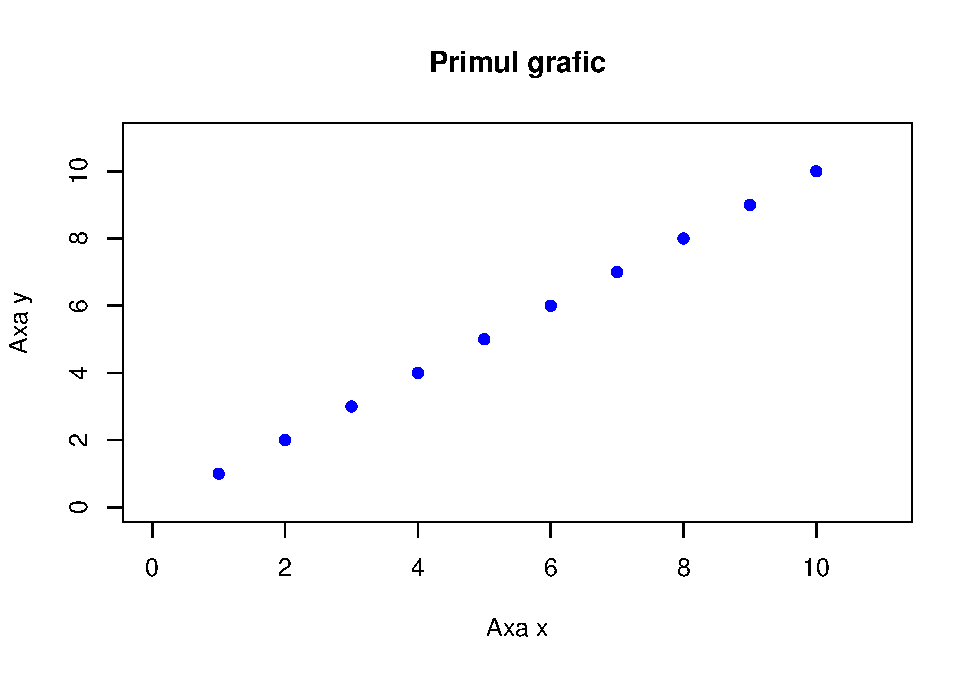
\includegraphics{Lab_2_files/figure-latex/unnamed-chunk-28-1} \end{center}

În afară de vectorii \texttt{x} și \texttt{y} toate celelalte argumente
sunt opționale, dacă nu sunt specificate atunci R-ul folosește valorile
prestabilite. De exemplu dacă nu specificăm limitele \texttt{xlim} și
\texttt{ylim}, R-ul calculează aceste limite astfel încât toate punctele
să fie încadrați în interiorul graficului.

\begin{rmdexercise}
Trasați următoarele diagrame de împrăștiere:

\texttt{x\ \textless{}-\ seq(0,\ 1,\ 0.1);\ plot(x,\ x\ -\ x\ *\ x\ +\ 2)}
\texttt{plot(x,\ x\ -\ x\ *\ x\ +\ 2,\ type\ =\ "l");\ plot(x,\ x\ -\ x\ *\ x\ +\ 2,\ type\ =\ "b",\ pch\ =\ 19)}
\end{rmdexercise}

Tipul de simbol pe care vrem să-l folosim atunci când trasăm un grafic
este specificat prin argumentul \texttt{pch}. Figura de mai jos ne
prezintă tipurile simboluri pe care atunci când atribuim argumentului
\texttt{pch} o valoare întreagă.

\begin{figure}

{\centering 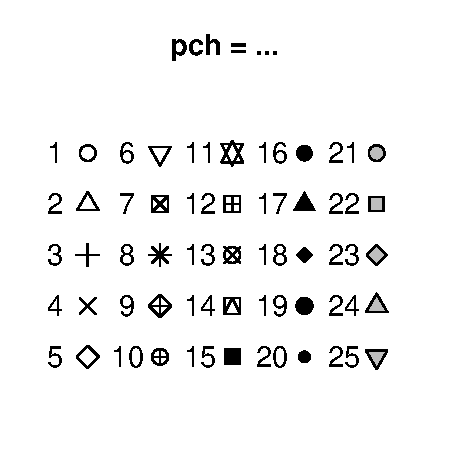
\includegraphics{Lab_2_files/figure-latex/unnamed-chunk-30-1} 

}

\caption{Tipurile de simboluri asociate parametrului pch.}\label{fig:unnamed-chunk-30}
\end{figure}

Următorul exemplu ilustrează câteva tipuri de simboluri:

\begin{center}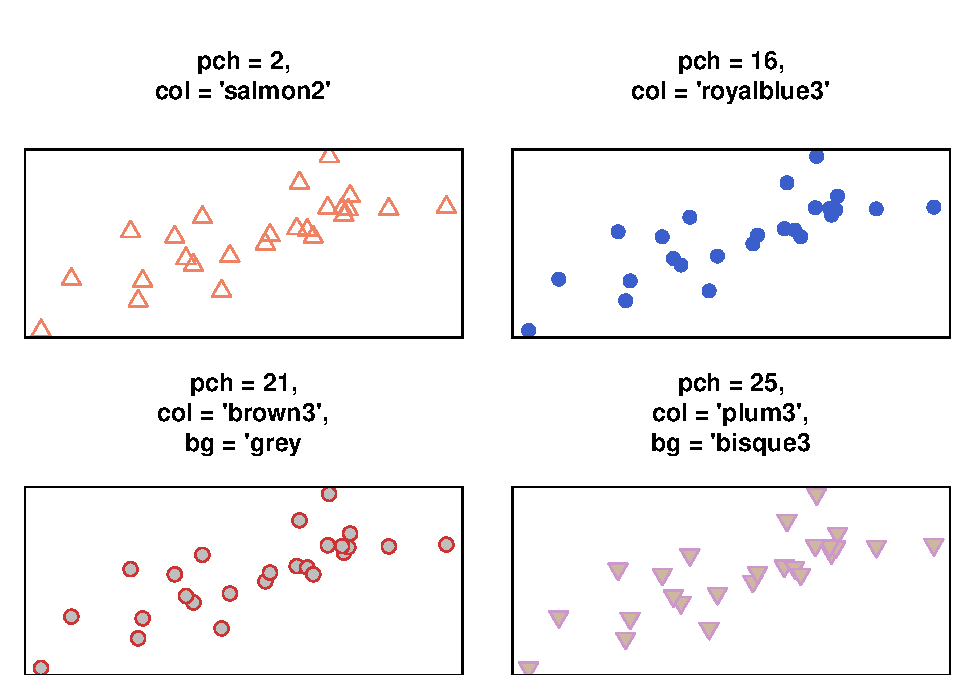
\includegraphics{Lab_2_files/figure-latex/unnamed-chunk-31-1} \end{center}

\begin{rmdexercise}
Considerăm următoarea funcție \(g:\mathbb{R}\to\mathbb{R}\),

\[
  g(x) = \left\{\begin{array}{ll}
              \sin^2(x)\log(x), & x>0\\
              \sin^2(x)x, & x\leq 0
  \end{array}\right.
\]

\begin{enumerate}
\def\labelenumi{\alph{enumi})}
\item
  Definiți funcția folosind comenzile \texttt{if-else} și
  \texttt{Vectorize} iar apoi folosind comanda \texttt{ifelse}.
\item
  Trasați graficul curbei pe intervalul \([-\pi, \pi]\).
\end{enumerate}
\end{rmdexercise}

\subsection{Culori}\label{culori}

Majoritatea funcțiilor de desenare au un argument în care pot specifica
culoarea elementelor pe care vrem să le trasăm, de cele mai multe ori
acesta este \texttt{col}. Cel mai ușor mod de a introduce o culoare este
prin specificarea numelui acesteia, de exemplu
\texttt{col\ =\ \textquotesingle{}red\textquotesingle{}} este culoarea
roșie. Figura 1 prezintă 144 de culori alese la întâmplare din totalul
de 657 câte există în R.

\begin{figure}

{\centering 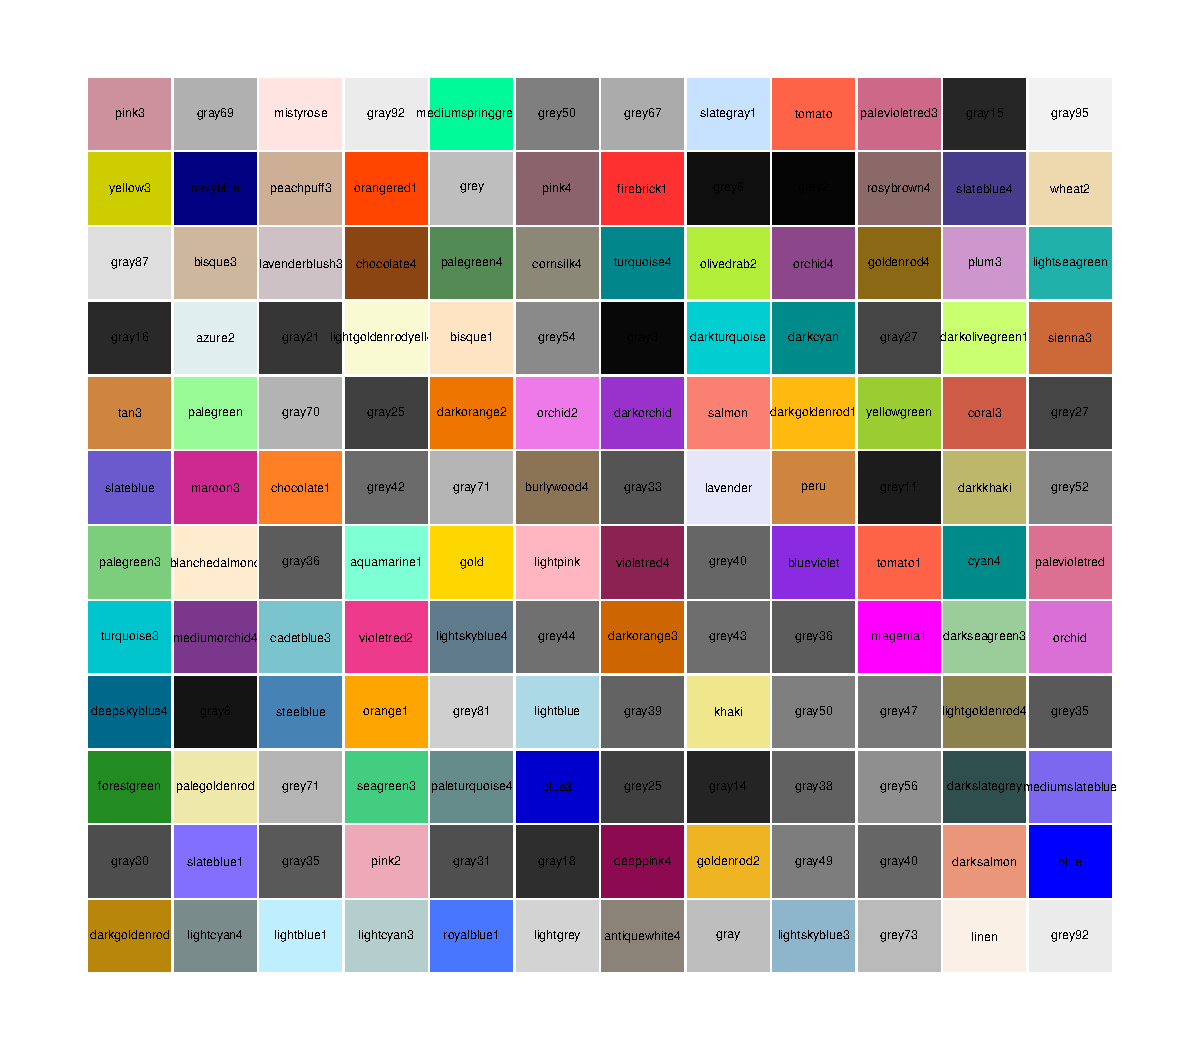
\includegraphics{Lab_2_files/figure-latex/randomcolors-1} 

}

\caption{144 de culori din totalul de 657 din R}\label{fig:randomcolors}
\end{figure}

Pentru a vedea toate culorile din R putem rula comanda
\texttt{colors()}.

\subsection{\texorpdfstring{Funcția
\texttt{hist}}{Funcția hist}}\label{functia-hist}

Histograma\footnote{Histograma este un estimator neparametric al
  densității.} reprezintă metoda grafică, cea mai comună, de
reprezentare a repartiției unui vector numeric. Pentru a crea o
histogramă în R folosim funcția \texttt{hist()} în care argumentul
principal este un vector numeric. Tabelul de mai jos prezintă
argumentele principale ale funcției \texttt{hist}.

\begin{longtable}[]{@{}ll@{}}
\caption{Argumentele funcției \texttt{hist()}}\tabularnewline
\toprule
\begin{minipage}[b]{0.18\columnwidth}\raggedright\strut
Argument\strut
\end{minipage} & \begin{minipage}[b]{0.67\columnwidth}\raggedright\strut
Descriere\strut
\end{minipage}\tabularnewline
\midrule
\endfirsthead
\toprule
\begin{minipage}[b]{0.18\columnwidth}\raggedright\strut
Argument\strut
\end{minipage} & \begin{minipage}[b]{0.67\columnwidth}\raggedright\strut
Descriere\strut
\end{minipage}\tabularnewline
\midrule
\endhead
\begin{minipage}[t]{0.18\columnwidth}\raggedright\strut
\texttt{x}\strut
\end{minipage} & \begin{minipage}[t]{0.67\columnwidth}\raggedright\strut
Vector de valori\strut
\end{minipage}\tabularnewline
\begin{minipage}[t]{0.18\columnwidth}\raggedright\strut
\texttt{breaks}\strut
\end{minipage} & \begin{minipage}[t]{0.67\columnwidth}\raggedright\strut
Cum să calculăm mărimea bin-urilor (vezi \texttt{?hist})\strut
\end{minipage}\tabularnewline
\begin{minipage}[t]{0.18\columnwidth}\raggedright\strut
\texttt{freq}\strut
\end{minipage} & \begin{minipage}[t]{0.67\columnwidth}\raggedright\strut
Opțiune pentru trasarea histogramei de frecvență și de probabilități,
\texttt{freq\ =\ TRUE} arată frecvențele, \texttt{freq\ =\ FALSE} arată
probabilitățile.\strut
\end{minipage}\tabularnewline
\begin{minipage}[t]{0.18\columnwidth}\raggedright\strut
\texttt{col}, \texttt{border}\strut
\end{minipage} & \begin{minipage}[t]{0.67\columnwidth}\raggedright\strut
Culoarea interioară a bin-urilor (\texttt{col}) și culoarea conturului
lor (\texttt{border})\strut
\end{minipage}\tabularnewline
\bottomrule
\end{longtable}

Putem crea o histogramă folosind setul de date \texttt{ChickWeight}
(\texttt{?ChickWeight})

\begin{Shaded}
\begin{Highlighting}[]
\KeywordTok{hist}\NormalTok{(}\DataTypeTok{x =}\NormalTok{ ChickWeight}\OperatorTok{$}\NormalTok{weight,}
     \DataTypeTok{main =} \StringTok{"Histograma greutatii gainilor"}\NormalTok{,}
     \DataTypeTok{xlab =} \StringTok{"Greutate"}\NormalTok{,}
     \DataTypeTok{ylab =} \StringTok{"Frecventa"}\NormalTok{,}
     \DataTypeTok{xlim =} \KeywordTok{c}\NormalTok{(}\DecValTok{0}\NormalTok{, }\DecValTok{500}\NormalTok{))}
\end{Highlighting}
\end{Shaded}

\begin{center}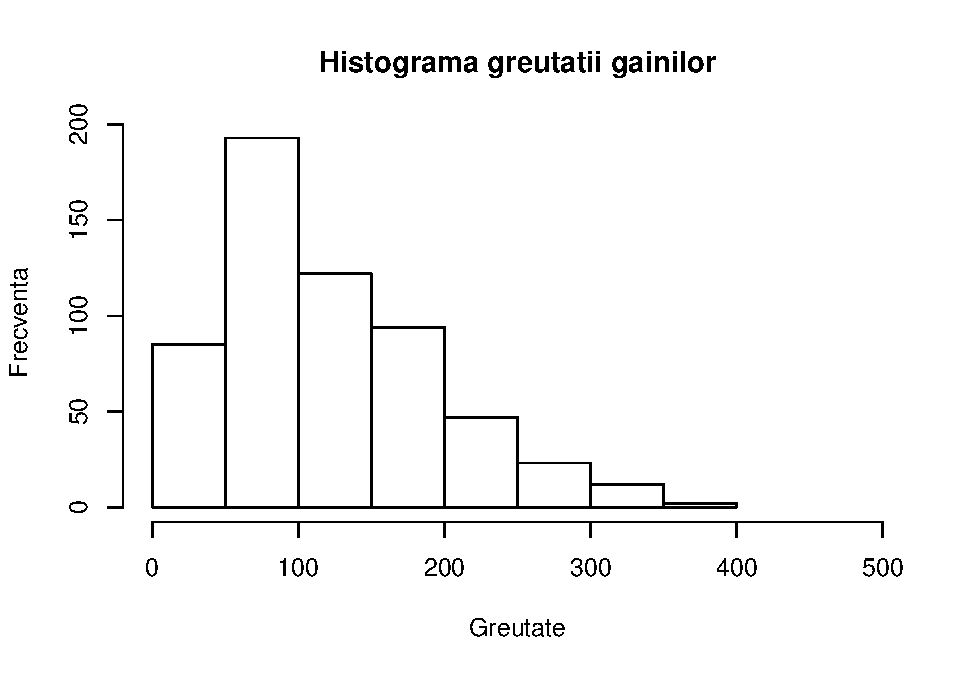
\includegraphics{Lab_2_files/figure-latex/unnamed-chunk-33-1} \end{center}

Putem modifica histograma de mai sus, schimbând numărul de bin-uri și
culoarea acestora:

\begin{Shaded}
\begin{Highlighting}[]
\KeywordTok{hist}\NormalTok{(}\DataTypeTok{x =}\NormalTok{ ChickWeight}\OperatorTok{$}\NormalTok{weight,}
     \DataTypeTok{main =} \StringTok{"O histograma mai colorata"}\NormalTok{,}
     \DataTypeTok{xlab =} \StringTok{"Greutate"}\NormalTok{,}
     \DataTypeTok{ylab =} \StringTok{"Frecventa"}\NormalTok{,}
     \DataTypeTok{breaks =} \DecValTok{20}\NormalTok{, }\CommentTok{# 20 Bins}
     \DataTypeTok{xlim =} \KeywordTok{c}\NormalTok{(}\DecValTok{0}\NormalTok{, }\DecValTok{500}\NormalTok{),}
     \DataTypeTok{col =} \StringTok{"skyblue"}\NormalTok{, }\CommentTok{# Culoarea de umplere}
     \DataTypeTok{border =} \StringTok{"royalblue3"}\NormalTok{) }\CommentTok{# Culoarea conturului}
\end{Highlighting}
\end{Shaded}

\begin{center}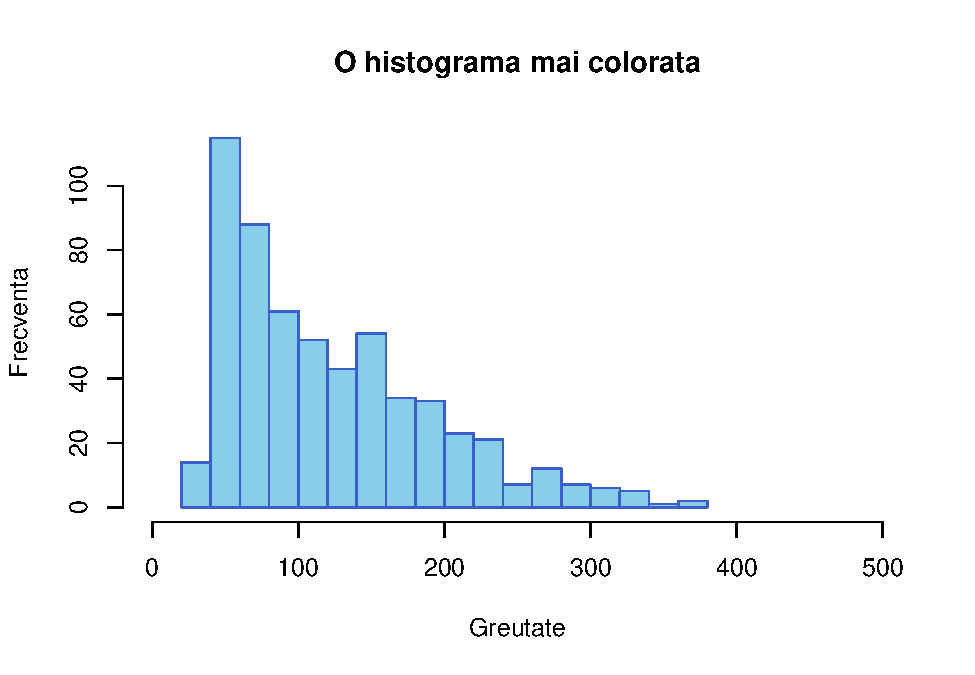
\includegraphics{Lab_2_files/figure-latex/unnamed-chunk-34-1} \end{center}

Dacă vrem să ilustrăm două histograme pe aceeași figură, pentru a
evidenția repartiția după două clase, putem folosi argumentul
\texttt{add\ =\ TRUE} la cel de-al doilea plot:

\begin{Shaded}
\begin{Highlighting}[]
\KeywordTok{hist}\NormalTok{(}\DataTypeTok{x =}\NormalTok{ ChickWeight}\OperatorTok{$}\NormalTok{weight[ChickWeight}\OperatorTok{$}\NormalTok{Diet }\OperatorTok{==}\StringTok{ }\DecValTok{1}\NormalTok{],}
     \DataTypeTok{main =} \StringTok{"Doua histograme pe acelasi grafic"}\NormalTok{,}
     \DataTypeTok{xlab =} \StringTok{"Greutate"}\NormalTok{,}
     \DataTypeTok{ylab =} \StringTok{"Frecventa"}\NormalTok{,}
     \DataTypeTok{breaks =} \DecValTok{20}\NormalTok{,}
     \DataTypeTok{xlim =} \KeywordTok{c}\NormalTok{(}\DecValTok{0}\NormalTok{, }\DecValTok{500}\NormalTok{),}
     \DataTypeTok{col =} \KeywordTok{gray}\NormalTok{(}\DecValTok{0}\NormalTok{, .}\DecValTok{5}\NormalTok{))}

\KeywordTok{hist}\NormalTok{(}\DataTypeTok{x =}\NormalTok{ ChickWeight}\OperatorTok{$}\NormalTok{weight[ChickWeight}\OperatorTok{$}\NormalTok{Diet }\OperatorTok{==}\StringTok{ }\DecValTok{2}\NormalTok{],}
     \DataTypeTok{breaks =} \DecValTok{30}\NormalTok{,}
     \DataTypeTok{add =} \OtherTok{TRUE}\NormalTok{, }\CommentTok{# Adauga graficul la cel de dinainte}
     \DataTypeTok{col =} \KeywordTok{gray}\NormalTok{(}\DecValTok{1}\NormalTok{, .}\DecValTok{8}\NormalTok{))}
\end{Highlighting}
\end{Shaded}

\begin{center}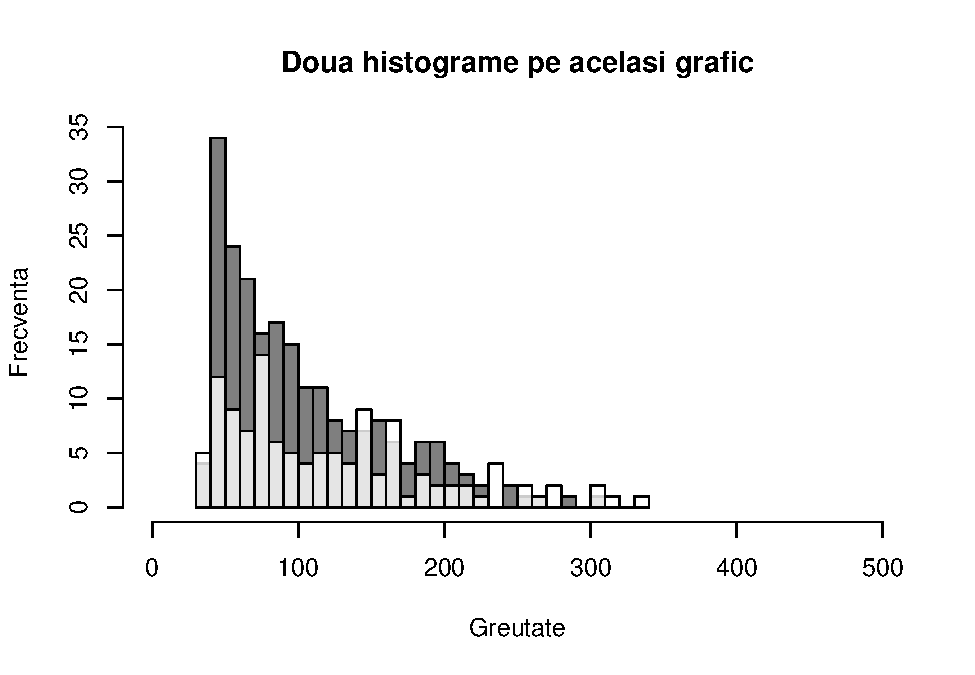
\includegraphics{Lab_2_files/figure-latex/unnamed-chunk-35-1} \end{center}

\subsection{\texorpdfstring{Funcția
\texttt{barplot}}{Funcția barplot}}\label{functia-barplot}

Funcția \texttt{barplot} este folosită în special atunci când avem de-a
face cu o variabilă discretă. Argumentul principal al funcției este
\texttt{height}, un vector numeric care va genera înălțimea fiecărei
bare. Pentru a adăuga nume sub fiecare bară putem folosi argumentul
\texttt{names.arg}.

De exemplu, folosind setul de date \texttt{mtcars} putem să afișăm
greutatea medie a mașinilor în funcție de numărul de cilindrii:

\begin{Shaded}
\begin{Highlighting}[]
\KeywordTok{par}\NormalTok{(}\DataTypeTok{mfrow =} \KeywordTok{c}\NormalTok{(}\DecValTok{1}\NormalTok{, }\DecValTok{2}\NormalTok{))}

\NormalTok{weight_cars =}\StringTok{ }\KeywordTok{aggregate}\NormalTok{(wt }\OperatorTok{~}\StringTok{ }\NormalTok{cyl, }
                        \DataTypeTok{data =}\NormalTok{ mtcars, }
                        \DataTypeTok{FUN =}\NormalTok{ mean)}

\KeywordTok{barplot}\NormalTok{(}\DataTypeTok{height =}\NormalTok{ weight_cars}\OperatorTok{$}\NormalTok{wt,}
        \DataTypeTok{names.arg =}\NormalTok{ weight_cars}\OperatorTok{$}\NormalTok{cyl,}
        \DataTypeTok{xlab =} \StringTok{"Numar de cilindrii"}\NormalTok{,}
        \DataTypeTok{ylab =} \StringTok{"Greutatea medie"}\NormalTok{,}
        \DataTypeTok{main =} \StringTok{"Greutatea medie dupa numarul de cilindrii}\CharTok{\textbackslash{}n}\StringTok{ Barplot vertical"}\NormalTok{,}
        \DataTypeTok{col =} \StringTok{"grey80"}\NormalTok{, }
        \DataTypeTok{cex.main =} \FloatTok{0.7}\NormalTok{)}

\KeywordTok{barplot}\NormalTok{(}\DataTypeTok{height =}\NormalTok{ weight_cars}\OperatorTok{$}\NormalTok{wt,}
        \DataTypeTok{names.arg =}\NormalTok{ weight_cars}\OperatorTok{$}\NormalTok{cyl,}
        \DataTypeTok{horiz =} \OtherTok{TRUE}\NormalTok{,}
        \DataTypeTok{ylab =} \StringTok{"Numar de cilindrii"}\NormalTok{,}
        \DataTypeTok{xlab =} \StringTok{"Greutatea medie"}\NormalTok{,}
        \DataTypeTok{main =} \StringTok{"Greutatea medie dupa numarul de cilindrii}\CharTok{\textbackslash{}n}\StringTok{ Barplot orizontal"}\NormalTok{,}
        \DataTypeTok{col =} \StringTok{"grey80"}\NormalTok{, }
        \DataTypeTok{cex.main =} \FloatTok{0.7}\NormalTok{)}
\end{Highlighting}
\end{Shaded}

\begin{center}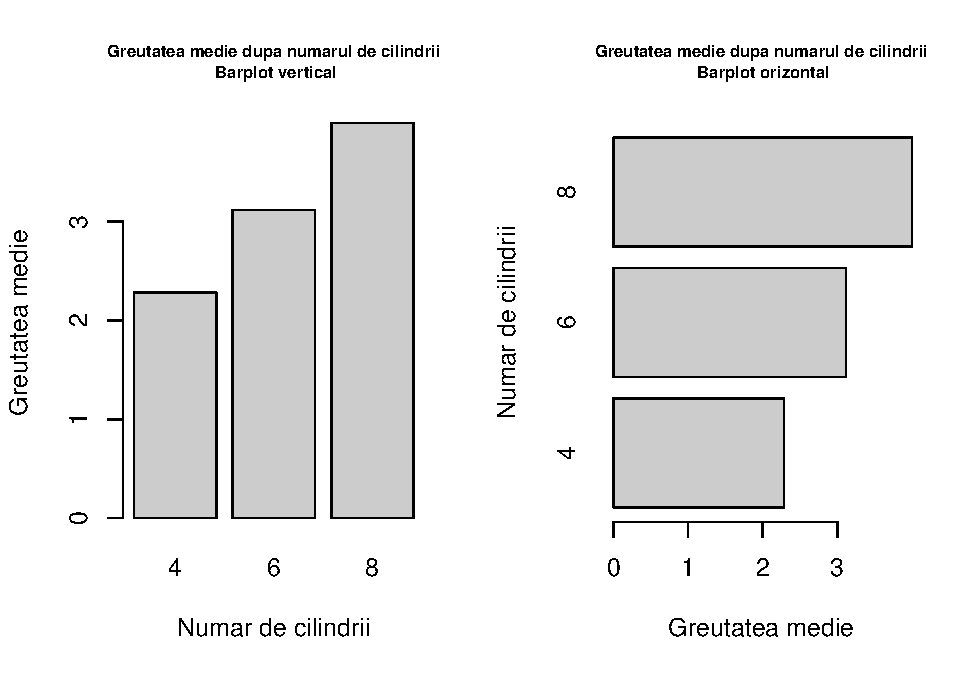
\includegraphics{Lab_2_files/figure-latex/unnamed-chunk-36-1} \end{center}

\begin{rmdexercise}
Folosind setul de date \texttt{ChickWeight} afișați, cu ajutorul
funcției \texttt{barplot}, greutatea medie a găinilor în raport cu
numărul de zile de la naștere.
\end{rmdexercise}

De asemenea putem crea un barplot clusterizat în funcție de mai multe
grupuri de date. De exemplu să presupunem că vrem să vedem dacă există
diferențe între greutatea medie a mașinilor (din setul de date
\texttt{mtcars}) care au transmisie manuală sau automată și numărul de
cilindrii.

\begin{Shaded}
\begin{Highlighting}[]
\CommentTok{# calculam greutatea medie dupa numarul de cilindrii si transmisie }
\NormalTok{carWeight_cyl_am =}\StringTok{ }\KeywordTok{aggregate}\NormalTok{(mtcars}\OperatorTok{$}\NormalTok{wt, }\DataTypeTok{by =} \KeywordTok{list}\NormalTok{(mtcars}\OperatorTok{$}\NormalTok{cyl, mtcars}\OperatorTok{$}\NormalTok{am), }\DataTypeTok{FUN =}\NormalTok{ mean) }

\CommentTok{# transformam rezultatul sub forma de matrice}
\NormalTok{carWeight_cyl_am =}\StringTok{ }\KeywordTok{as.matrix}\NormalTok{(carWeight_cyl_am)}
\NormalTok{carWeight_cyl_am}
\NormalTok{     Group.}\DecValTok{1}\NormalTok{ Group.}\DecValTok{2}\NormalTok{        x}
\NormalTok{[}\DecValTok{1}\NormalTok{,]       }\DecValTok{4}       \DecValTok{0} \FloatTok{2.935000}
\NormalTok{[}\DecValTok{2}\NormalTok{,]       }\DecValTok{6}       \DecValTok{0} \FloatTok{3.388750}
\NormalTok{[}\DecValTok{3}\NormalTok{,]       }\DecValTok{8}       \DecValTok{0} \FloatTok{4.104083}
\NormalTok{[}\DecValTok{4}\NormalTok{,]       }\DecValTok{4}       \DecValTok{1} \FloatTok{2.042250}
\NormalTok{[}\DecValTok{5}\NormalTok{,]       }\DecValTok{6}       \DecValTok{1} \FloatTok{2.755000}
\NormalTok{[}\DecValTok{6}\NormalTok{,]       }\DecValTok{8}       \DecValTok{1} \FloatTok{3.370000}

\CommentTok{# aducem la forma necesara pentru barplot}
\NormalTok{carWeight =}\StringTok{ }\KeywordTok{matrix}\NormalTok{(carWeight_cyl_am[,}\DecValTok{3}\NormalTok{], }\DataTypeTok{nrow =} \DecValTok{3}\NormalTok{)}
\KeywordTok{colnames}\NormalTok{(carWeight) =}\StringTok{ }\KeywordTok{unique}\NormalTok{(carWeight_cyl_am[,}\DecValTok{2}\NormalTok{])}
\KeywordTok{rownames}\NormalTok{(carWeight) =}\StringTok{ }\KeywordTok{unique}\NormalTok{(carWeight_cyl_am[, }\DecValTok{1}\NormalTok{])}

\NormalTok{carWeight =}\StringTok{ }\KeywordTok{t}\NormalTok{(carWeight)}

\KeywordTok{barplot}\NormalTok{(carWeight, }
        \DataTypeTok{beside =} \OtherTok{TRUE}\NormalTok{,}
        \DataTypeTok{legend.text =} \OtherTok{TRUE}\NormalTok{, }
        \DataTypeTok{col =} \KeywordTok{c}\NormalTok{(}\StringTok{"royalblue3"}\NormalTok{, }\StringTok{"brown3"}\NormalTok{),}
        \DataTypeTok{main =} \StringTok{"Greutatea medie a masinilor dupa numarul de cilindrii si transmisie"}\NormalTok{,}
        \DataTypeTok{xlab =} \StringTok{"Numar de cilindrii"}\NormalTok{,}
        \DataTypeTok{ylab =} \StringTok{"Greutatea medie"}\NormalTok{)}
\end{Highlighting}
\end{Shaded}

\begin{center}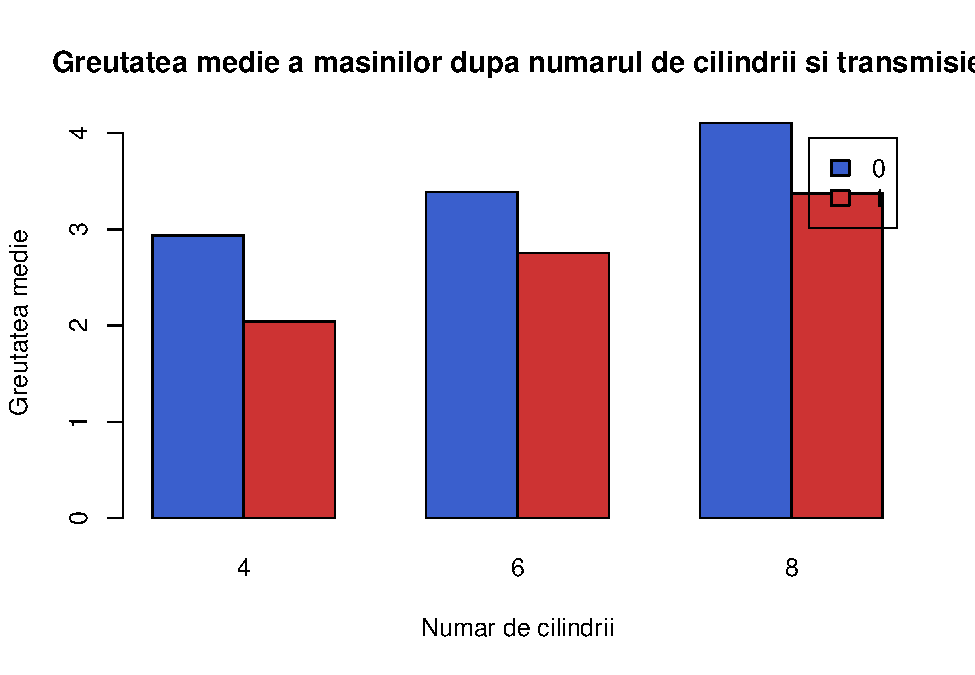
\includegraphics{Lab_2_files/figure-latex/unnamed-chunk-38-1} \end{center}

\subsection{\texorpdfstring{Funcția
\texttt{boxplot}}{Funcția boxplot}}\label{functia-boxplot}

Pentru a vedea cât de bine sunt repartizate datele în setul de date
putem folosi funcția \texttt{boxplot} (box and whisker plot - cutie cu
mustăți). Această funcție prezintă într-o manieră compactă modul în care
este repartizată o variabilă. Această metodă grafică prezintă
principalii indicatori de poziție ai variabilei studiate: cuartilele de
ordin 1 și 3 (\(Q_1\), \(Q_3\)) care delimitează cutia
(\(IQR = Q_3-Q_1\)) și cuartila de ordin 2 sau mediana (linia din
interiorul cutiei). Mustățile sunt calculate în modul următor: mustața
superioară este determinată de valoarea celei mai mari observații care
este mai mică sau egală cu \(Q_3 + 1.5 IQR\) iar mustața inferioară este
valoarea celei mai mici observații mai mari sau egale cu \(Q_1-1.5IQR\).
Valorile din afara cutiei cu mustăți se numesc valori aberante.

Principalele argumente ale funcției \texttt{boxplot} se regăsesc în
tabelul următor, pentru mai multe detalii apelați \texttt{?boxplot}.

\begin{longtable}[]{@{}ll@{}}
\caption{Principalele argumente ale functiei boxplot.}\tabularnewline
\toprule
\begin{minipage}[b]{0.18\columnwidth}\raggedright\strut
Argument\strut
\end{minipage} & \begin{minipage}[b]{0.67\columnwidth}\raggedright\strut
Descriere\strut
\end{minipage}\tabularnewline
\midrule
\endfirsthead
\toprule
\begin{minipage}[b]{0.18\columnwidth}\raggedright\strut
Argument\strut
\end{minipage} & \begin{minipage}[b]{0.67\columnwidth}\raggedright\strut
Descriere\strut
\end{minipage}\tabularnewline
\midrule
\endhead
\begin{minipage}[t]{0.18\columnwidth}\raggedright\strut
\texttt{formula}\strut
\end{minipage} & \begin{minipage}[t]{0.67\columnwidth}\raggedright\strut
O formulă de tip \texttt{y\ \textasciitilde{}\ grp}, unde \texttt{y}
este variabila investigată iar \texttt{grp} este variabila care descrie
grupurile după care vrem să trasăm grafiul\strut
\end{minipage}\tabularnewline
\begin{minipage}[t]{0.18\columnwidth}\raggedright\strut
\texttt{data}\strut
\end{minipage} & \begin{minipage}[t]{0.67\columnwidth}\raggedright\strut
Un data frame (sau listă) în care variabilele din formulă sunt
definite\strut
\end{minipage}\tabularnewline
\begin{minipage}[t]{0.18\columnwidth}\raggedright\strut
\texttt{subset}\strut
\end{minipage} & \begin{minipage}[t]{0.67\columnwidth}\raggedright\strut
Un vector care specifică o submulțime a observațiilor\strut
\end{minipage}\tabularnewline
\begin{minipage}[t]{0.18\columnwidth}\raggedright\strut
\texttt{x}\strut
\end{minipage} & \begin{minipage}[t]{0.67\columnwidth}\raggedright\strut
Un vector care specifică valorile ce urmează să fie trasate\strut
\end{minipage}\tabularnewline
\begin{minipage}[t]{0.18\columnwidth}\raggedright\strut
\texttt{horizontal}\strut
\end{minipage} & \begin{minipage}[t]{0.67\columnwidth}\raggedright\strut
O valoare logică care indică dacă trasăm boxplot-urile vertical
(\texttt{FALSE}) sau orizontal (\texttt{TRUE})\strut
\end{minipage}\tabularnewline
\begin{minipage}[t]{0.18\columnwidth}\raggedright\strut
\texttt{add}\strut
\end{minipage} & \begin{minipage}[t]{0.67\columnwidth}\raggedright\strut
O valoare logică prin care se permite adăugarea graficului la unul deja
existent\strut
\end{minipage}\tabularnewline
\bottomrule
\end{longtable}

Următorul exemplu ne prezintă relația dintre consum (\texttt{mpg}) și
numărul de cilindrii (\texttt{cyl}) în cazul mașinilor din setul de date
\texttt{mtcars}.

\begin{Shaded}
\begin{Highlighting}[]
\KeywordTok{boxplot}\NormalTok{(mpg }\OperatorTok{~}\StringTok{ }\NormalTok{cyl, }
        \DataTypeTok{data =}\NormalTok{ mtcars, }
        \DataTypeTok{xlab =} \StringTok{"Numar de cilindrii"}\NormalTok{,}
        \DataTypeTok{ylab =} \StringTok{"Mile pe galon"}\NormalTok{, }
        \DataTypeTok{main =} \StringTok{"Consumul in functie de numarul de cilindrii"}\NormalTok{)}
\end{Highlighting}
\end{Shaded}

\begin{center}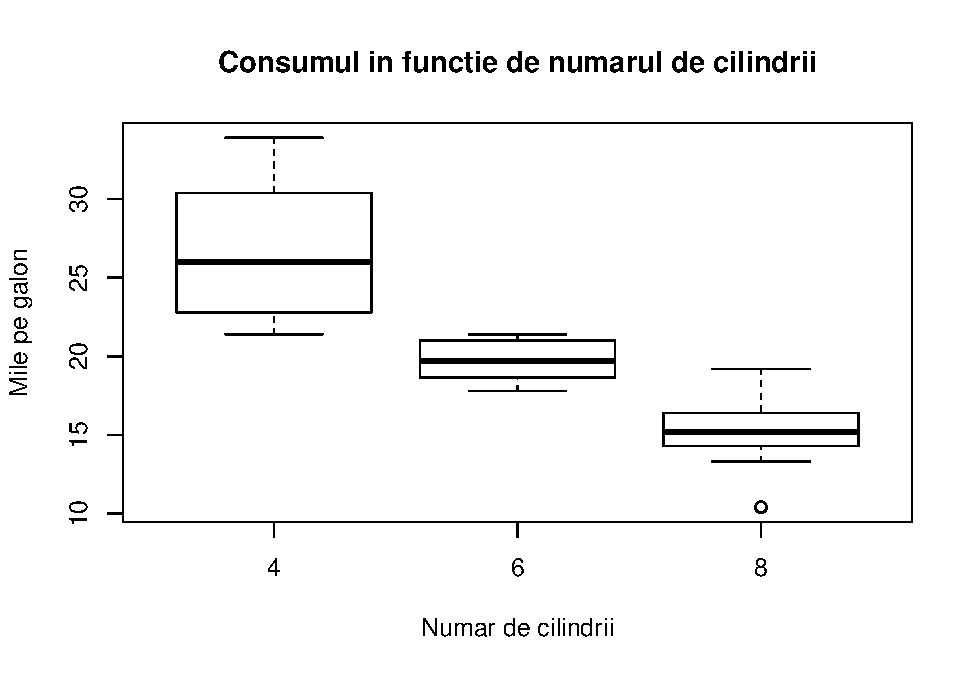
\includegraphics{Lab_2_files/figure-latex/unnamed-chunk-39-1} \end{center}

Putem să vedem această relație și în raport cu tipul de transmisie.

\begin{Shaded}
\begin{Highlighting}[]
\KeywordTok{boxplot}\NormalTok{(mpg }\OperatorTok{~}\StringTok{ }\NormalTok{cyl, }
        \DataTypeTok{data =}\NormalTok{ mtcars, }
        \DataTypeTok{subset =}\NormalTok{ am }\OperatorTok{==}\StringTok{ }\DecValTok{0}\NormalTok{,}
        \DataTypeTok{boxwex =} \FloatTok{0.25}\NormalTok{, }
        \DataTypeTok{at =} \DecValTok{1}\OperatorTok{:}\DecValTok{3} \OperatorTok{-}\StringTok{ }\FloatTok{0.2}\NormalTok{,}
        \DataTypeTok{col =} \StringTok{"darkgrey"}\NormalTok{,}
        \DataTypeTok{xlab =} \StringTok{"Numar de cilindrii"}\NormalTok{,}
        \DataTypeTok{ylab =} \StringTok{"Mile pe galon"}\NormalTok{, }
        \DataTypeTok{main =} \StringTok{"Consumul dupa de numarul de cilindrii si transmisie"}\NormalTok{,}
        \DataTypeTok{xlim =} \KeywordTok{c}\NormalTok{(}\FloatTok{0.5}\NormalTok{, }\FloatTok{3.5}\NormalTok{), }
        \DataTypeTok{ylim =} \KeywordTok{c}\NormalTok{(}\DecValTok{0}\NormalTok{, }\DecValTok{35}\NormalTok{),}
        \DataTypeTok{yaxs =} \StringTok{"i"}\NormalTok{)}

\KeywordTok{boxplot}\NormalTok{(mpg }\OperatorTok{~}\StringTok{ }\NormalTok{cyl, }
        \DataTypeTok{data =}\NormalTok{ mtcars, }
        \DataTypeTok{subset =}\NormalTok{ am }\OperatorTok{==}\StringTok{ }\DecValTok{1}\NormalTok{,}
        \DataTypeTok{add =} \OtherTok{TRUE}\NormalTok{,}
        \DataTypeTok{boxwex =} \FloatTok{0.25}\NormalTok{, }
        \DataTypeTok{at =} \DecValTok{1}\OperatorTok{:}\DecValTok{3} \OperatorTok{+}\StringTok{ }\FloatTok{0.2}\NormalTok{,}
        \DataTypeTok{col =} \StringTok{"brown3"}\NormalTok{)}

\KeywordTok{legend}\NormalTok{(}\StringTok{"bottomright"}\NormalTok{ ,}\KeywordTok{c}\NormalTok{(}\StringTok{"Manuala"}\NormalTok{, }\StringTok{"Automata"}\NormalTok{),}
       \DataTypeTok{fill =} \KeywordTok{c}\NormalTok{(}\StringTok{"lightgray"}\NormalTok{, }\StringTok{"brown3"}\NormalTok{), }\DataTypeTok{bty =} \StringTok{"n"}\NormalTok{)}
\end{Highlighting}
\end{Shaded}

\begin{center}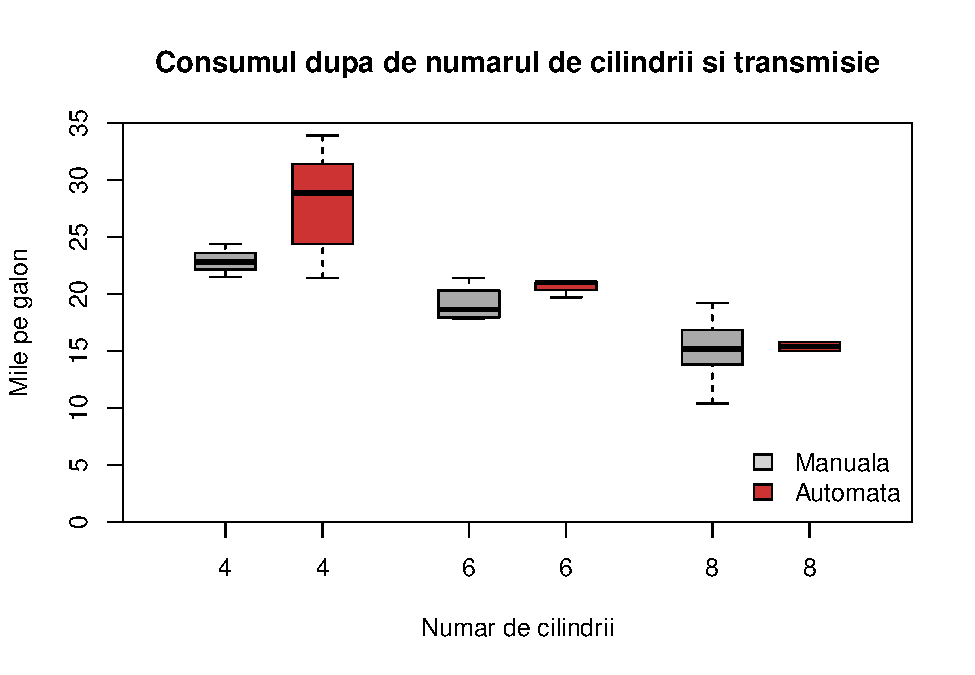
\includegraphics{Lab_2_files/figure-latex/unnamed-chunk-40-1} \end{center}

\subsection{Funcții pentru adăugarea unor elemente la un
grafic}\label{functii-pentru-adaugarea-unor-elemente-la-un-grafic}

Funcțiile (low-level) din această secțiune sunt folosite pentru a adăuga
elemente, de tipul linii, puncte, text la un grafic deja existent.

\begin{longtable}[]{@{}ll@{}}
\caption{Functii low-level uzuale}\tabularnewline
\toprule
Funcția & rezultatul\tabularnewline
\midrule
\endfirsthead
\toprule
Funcția & rezultatul\tabularnewline
\midrule
\endhead
\texttt{points(x,\ y)} & Adaugă puncte la un grafic.\tabularnewline
\texttt{abline()}, \texttt{segments()} & Adaugă linii sau segmente la un
grafic existent.\tabularnewline
\texttt{arrows()} & Adaugă săgeți.\tabularnewline
\texttt{curve()} & Adaugă o curbă care reprezintă graficul unei
funcții.\tabularnewline
\texttt{rect()},\texttt{polygon()} & Adaugă un dreptunghi sau un poligon
oarecare.\tabularnewline
\texttt{text()}, \texttt{mtext()} & Adaugă text la o
figură.\tabularnewline
\texttt{legend()} & Adaugă legenda.\tabularnewline
\texttt{axis()} & Adaugă o axă.\tabularnewline
\bottomrule
\end{longtable}

Pentru a adăuga noi puncte la un grafic deja existent putem folosi
funcție \texttt{points()}. Pentru a vedea toate argumentele acestei
funcții apelați \texttt{?points}.

Să considerăm următorul exemplu în care trasăm diagrama de împrăștiere
după consum (\texttt{mpg}) și putere (\texttt{hp}) pentru mașinile din
setul de date \texttt{mtcars} în raport cu tipul de transmisie.

\begin{Shaded}
\begin{Highlighting}[]
\KeywordTok{plot}\NormalTok{(}\DataTypeTok{x =}\NormalTok{ mtcars}\OperatorTok{$}\NormalTok{mpg[mtcars}\OperatorTok{$}\NormalTok{am }\OperatorTok{==}\StringTok{ }\DecValTok{0}\NormalTok{], }
     \DataTypeTok{y =}\NormalTok{ mtcars}\OperatorTok{$}\NormalTok{hp[mtcars}\OperatorTok{$}\NormalTok{am }\OperatorTok{==}\StringTok{ }\DecValTok{0}\NormalTok{], }
     \DataTypeTok{xlab =} \StringTok{"Mile pe galon"}\NormalTok{,}
     \DataTypeTok{ylab =} \StringTok{"Cai putere"}\NormalTok{, }
     \DataTypeTok{main =} \StringTok{"Consum vs Cai putere dupa transmisie"}\NormalTok{,}
     \DataTypeTok{pch =} \DecValTok{16}\NormalTok{, }
     \DataTypeTok{col =} \StringTok{"darkgrey"}\NormalTok{)}

\KeywordTok{points}\NormalTok{(}\DataTypeTok{x =}\NormalTok{ mtcars}\OperatorTok{$}\NormalTok{mpg[mtcars}\OperatorTok{$}\NormalTok{am }\OperatorTok{==}\StringTok{ }\DecValTok{1}\NormalTok{], }
      \DataTypeTok{y =}\NormalTok{ mtcars}\OperatorTok{$}\NormalTok{hp[mtcars}\OperatorTok{$}\NormalTok{am }\OperatorTok{==}\StringTok{ }\DecValTok{1}\NormalTok{], }
      \DataTypeTok{pch =} \DecValTok{16}\NormalTok{, }
      \DataTypeTok{col =} \StringTok{"brown3"}\NormalTok{)}
\end{Highlighting}
\end{Shaded}

\begin{center}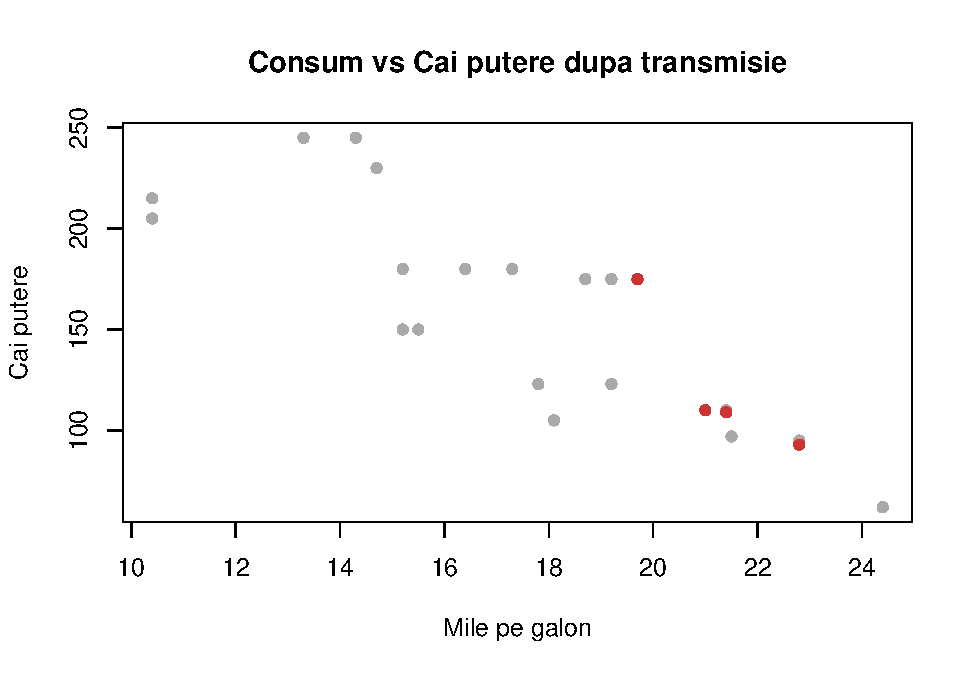
\includegraphics{Lab_2_files/figure-latex/unnamed-chunk-41-1} \end{center}

Dacă vrem să adăugăm linii drepte la un grafic putem folosi comanda
\texttt{abline()} sau \texttt{segments()}. De exemplu în figura de mai
sus vrem să adăugăm o linie verticală și una orizontală care să marcheze
media variabilelor de pe axa x și y.

\begin{Shaded}
\begin{Highlighting}[]
\KeywordTok{plot}\NormalTok{(}\DataTypeTok{x =}\NormalTok{ mtcars}\OperatorTok{$}\NormalTok{mpg, }
     \DataTypeTok{y =}\NormalTok{ mtcars}\OperatorTok{$}\NormalTok{hp, }
     \DataTypeTok{xlab =} \StringTok{"Mile pe galon"}\NormalTok{,}
     \DataTypeTok{ylab =} \StringTok{"Cai putere"}\NormalTok{, }
     \DataTypeTok{main =} \StringTok{"Consum vs Cai putere"}\NormalTok{,}
     \DataTypeTok{pch =} \DecValTok{16}\NormalTok{, }
     \DataTypeTok{col =} \StringTok{"darkgrey"}\NormalTok{)}

\KeywordTok{abline}\NormalTok{(}\DataTypeTok{h =} \KeywordTok{mean}\NormalTok{(mtcars}\OperatorTok{$}\NormalTok{hp), }\DataTypeTok{lty =} \DecValTok{2}\NormalTok{)}
\KeywordTok{abline}\NormalTok{(}\DataTypeTok{v =} \KeywordTok{mean}\NormalTok{(mtcars}\OperatorTok{$}\NormalTok{mpg), }\DataTypeTok{lty =} \DecValTok{2}\NormalTok{)}
\end{Highlighting}
\end{Shaded}

\begin{center}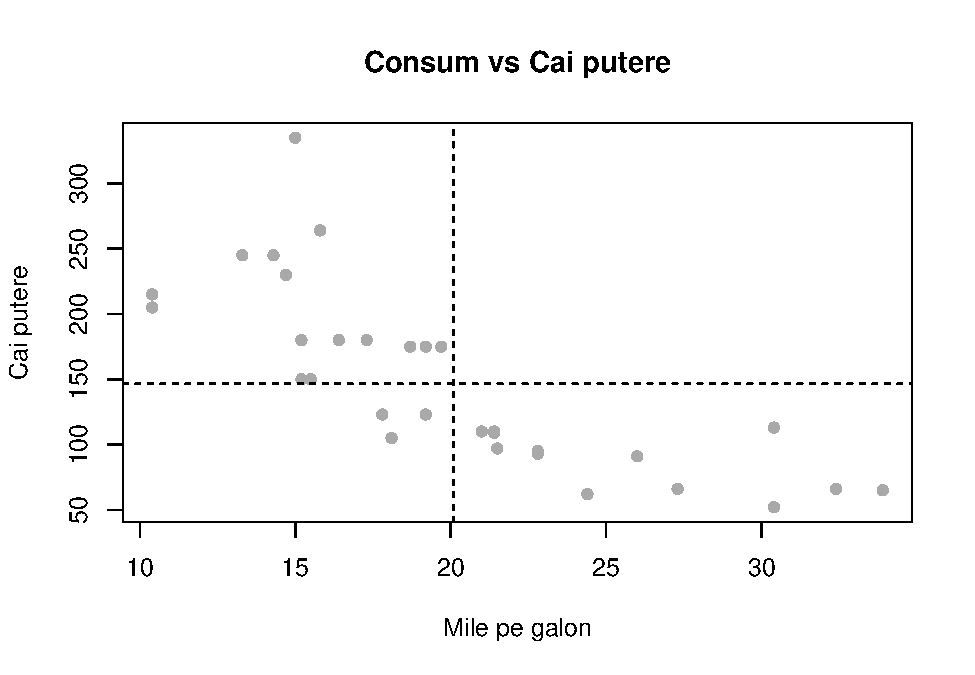
\includegraphics{Lab_2_files/figure-latex/unnamed-chunk-42-1} \end{center}

Pentru a adăuga numele mașinilor cu transmisie automată în fiecare punct
putem folosi comanda \texttt{text()}. Argumentele principale ale acestei
funcții sunt \texttt{x}, \texttt{y} care descriu coordonatele
etichetelor și \texttt{labels} care reprezintă etichetele.

\begin{Shaded}
\begin{Highlighting}[]
\KeywordTok{plot}\NormalTok{(}\DataTypeTok{x =}\NormalTok{ mtcars}\OperatorTok{$}\NormalTok{mpg, }
     \DataTypeTok{y =}\NormalTok{ mtcars}\OperatorTok{$}\NormalTok{hp, }
     \DataTypeTok{xlab =} \StringTok{"Mile pe galon"}\NormalTok{,}
     \DataTypeTok{ylab =} \StringTok{"Cai putere"}\NormalTok{, }
     \DataTypeTok{main =} \StringTok{"Consum vs Cai putere"}\NormalTok{,}
     \DataTypeTok{pch =} \DecValTok{16}\NormalTok{, }
     \DataTypeTok{col =} \StringTok{"darkgrey"}\NormalTok{)}

\KeywordTok{abline}\NormalTok{(}\DataTypeTok{h =} \KeywordTok{mean}\NormalTok{(mtcars}\OperatorTok{$}\NormalTok{hp), }\DataTypeTok{lty =} \DecValTok{2}\NormalTok{)}
\KeywordTok{abline}\NormalTok{(}\DataTypeTok{v =} \KeywordTok{mean}\NormalTok{(mtcars}\OperatorTok{$}\NormalTok{mpg), }\DataTypeTok{lty =} \DecValTok{2}\NormalTok{)}

\KeywordTok{text}\NormalTok{(}\DataTypeTok{x =}\NormalTok{ mtcars}\OperatorTok{$}\NormalTok{mpg[mtcars}\OperatorTok{$}\NormalTok{am }\OperatorTok{==}\StringTok{ }\DecValTok{1}\NormalTok{], }
     \DataTypeTok{y =}\NormalTok{ mtcars}\OperatorTok{$}\NormalTok{hp[mtcars}\OperatorTok{$}\NormalTok{am }\OperatorTok{==}\StringTok{ }\DecValTok{1}\NormalTok{],}
     \DataTypeTok{labels =} \KeywordTok{rownames}\NormalTok{(mtcars[mtcars}\OperatorTok{$}\NormalTok{am }\OperatorTok{==}\StringTok{ }\DecValTok{1}\NormalTok{, ]), }
     \DataTypeTok{pos =} \DecValTok{3}\NormalTok{, }
     \DataTypeTok{cex =} \FloatTok{0.5}\NormalTok{)}
\end{Highlighting}
\end{Shaded}

\begin{center}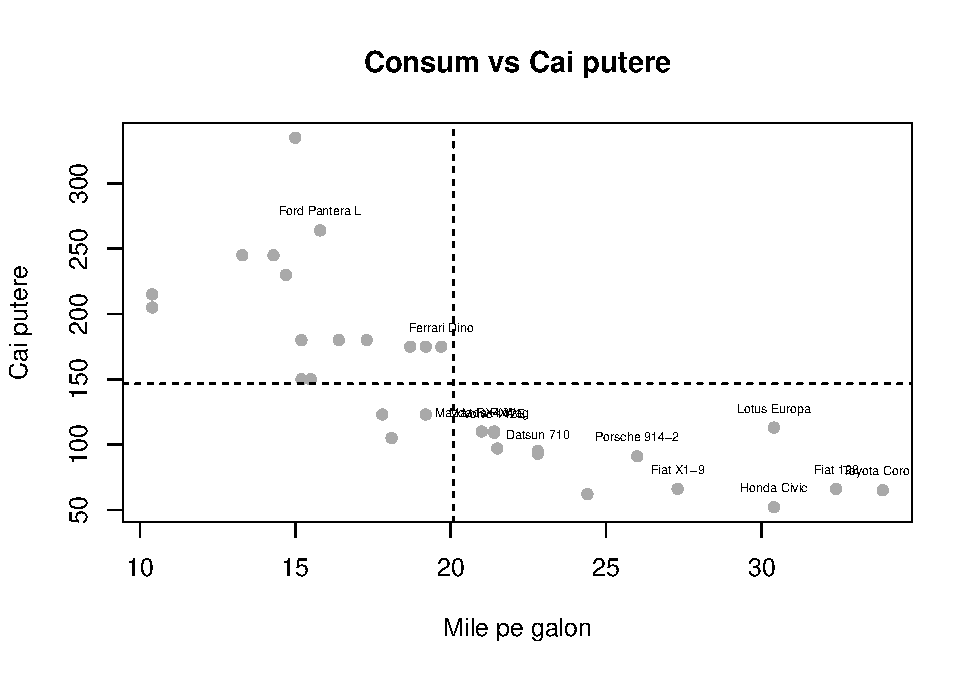
\includegraphics{Lab_2_files/figure-latex/unnamed-chunk-43-1} \end{center}

Funcția \texttt{curve()} permite trasarea/adăugarea unei linii care
descrie o funcție. Printre argumentele funcției regăsim \texttt{expr}
care reprezintă expresia funcției care depinde de \texttt{x} (se pot
folosi și funcții customizate), \texttt{from,\ to} care reprezintă
intervalul de valori pentru \texttt{x} și \texttt{add} care permite
adăugarea unei curbe la un grafic existent.

\begin{Shaded}
\begin{Highlighting}[]
\KeywordTok{curve}\NormalTok{(}\DataTypeTok{expr =} \KeywordTok{sin}\NormalTok{(x),}
      \DataTypeTok{from =} \DecValTok{0}\NormalTok{,}
      \DataTypeTok{to =} \DecValTok{2}\OperatorTok{*}\NormalTok{pi, }
      \DataTypeTok{ylab =} \StringTok{""}\NormalTok{, }
      \DataTypeTok{main =} \StringTok{"Graficul functiei sin si cos"}\NormalTok{,}
      \DataTypeTok{col =} \StringTok{"red"}\NormalTok{)}

\KeywordTok{curve}\NormalTok{(}\DataTypeTok{expr =} \KeywordTok{cos}\NormalTok{(x),}
      \DataTypeTok{from =} \DecValTok{0}\NormalTok{,}
      \DataTypeTok{to =} \DecValTok{2}\OperatorTok{*}\NormalTok{pi,}
      \DataTypeTok{add =} \OtherTok{TRUE}\NormalTok{,}
      \DataTypeTok{col =} \StringTok{"blue"}\NormalTok{, }
      \DataTypeTok{lty =} \DecValTok{2}\NormalTok{)}
\end{Highlighting}
\end{Shaded}

\begin{center}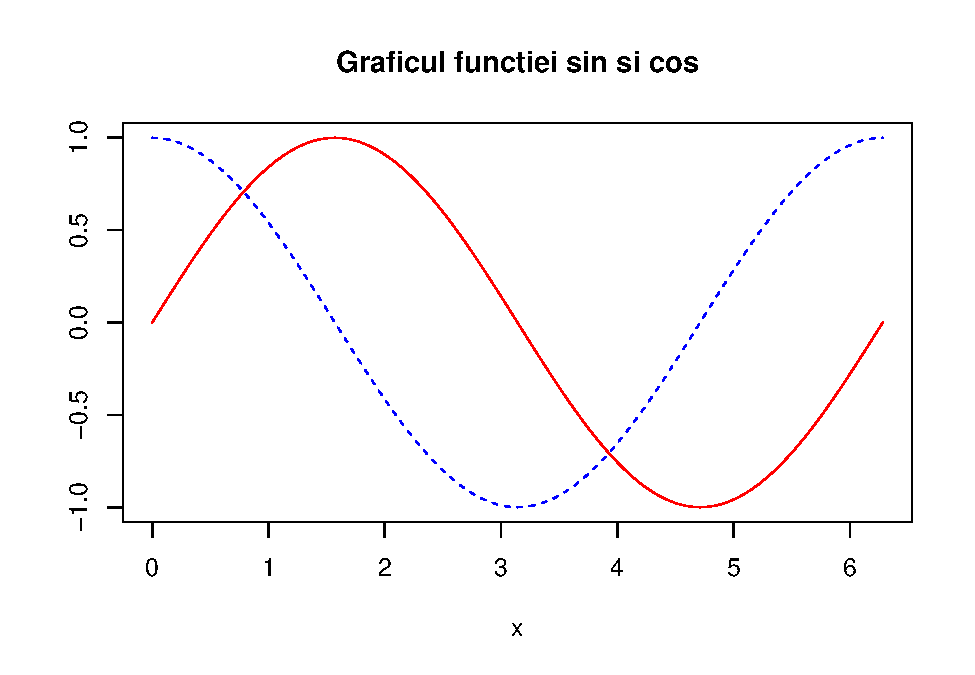
\includegraphics{Lab_2_files/figure-latex/unnamed-chunk-44-1} \end{center}

Atunci când vrem să adăugăm o legendă la un grafic folosim funcția
\texttt{legend()}. Argumentele acestei funcții se regăsesc în tabelul de
mai jos.

\begin{longtable}[]{@{}ll@{}}
\caption{Argumentele functiei legend()}\tabularnewline
\toprule
\begin{minipage}[b]{0.14\columnwidth}\raggedright\strut
Argument\strut
\end{minipage} & \begin{minipage}[b]{0.71\columnwidth}\raggedright\strut
Rezultat\strut
\end{minipage}\tabularnewline
\midrule
\endfirsthead
\toprule
\begin{minipage}[b]{0.14\columnwidth}\raggedright\strut
Argument\strut
\end{minipage} & \begin{minipage}[b]{0.71\columnwidth}\raggedright\strut
Rezultat\strut
\end{minipage}\tabularnewline
\midrule
\endhead
\begin{minipage}[t]{0.14\columnwidth}\raggedright\strut
\texttt{x,\ y}\strut
\end{minipage} & \begin{minipage}[t]{0.71\columnwidth}\raggedright\strut
Coordonatele legendei - de exemplu, \texttt{x\ =\ 0,\ y\ =\ 0} va pune
legenda la coordonatele (0, 0). Alternativ, putem indica poziția unde
vrem legenda (i.e. \texttt{"topright"}, \texttt{"topleft"}).\strut
\end{minipage}\tabularnewline
\begin{minipage}[t]{0.14\columnwidth}\raggedright\strut
\texttt{legend}\strut
\end{minipage} & \begin{minipage}[t]{0.71\columnwidth}\raggedright\strut
Un vector de caractere care precizează textul care vrem să apară în
legendă.\strut
\end{minipage}\tabularnewline
\begin{minipage}[t]{0.14\columnwidth}\raggedright\strut
\texttt{pch,\ lty,\ lwd,\ col,\ pt.bg,\ ...}\strut
\end{minipage} & \begin{minipage}[t]{0.71\columnwidth}\raggedright\strut
Argumente grafice adiționale (pentru detalii apelați
\texttt{?legend}).\strut
\end{minipage}\tabularnewline
\bottomrule
\end{longtable}

Ca exemplu prim să considerăm graficele de funcții de mai sus la care
vrem să specificăm care grafic corespunde funcției \(sin\) și care
funcției \(cos\):

\begin{Shaded}
\begin{Highlighting}[]
\KeywordTok{curve}\NormalTok{(}\DataTypeTok{expr =} \KeywordTok{sin}\NormalTok{(x),}
      \DataTypeTok{from =} \DecValTok{0}\NormalTok{,}
      \DataTypeTok{to =} \DecValTok{2}\OperatorTok{*}\NormalTok{pi, }
      \DataTypeTok{ylab =} \StringTok{""}\NormalTok{, }
      \DataTypeTok{main =} \StringTok{"Graficul functiei sin si cos"}\NormalTok{,}
      \DataTypeTok{col =} \StringTok{"red"}\NormalTok{)}

\KeywordTok{curve}\NormalTok{(}\DataTypeTok{expr =} \KeywordTok{cos}\NormalTok{(x),}
      \DataTypeTok{from =} \DecValTok{0}\NormalTok{,}
      \DataTypeTok{to =} \DecValTok{2}\OperatorTok{*}\NormalTok{pi,}
      \DataTypeTok{add =} \OtherTok{TRUE}\NormalTok{,}
      \DataTypeTok{col =} \StringTok{"blue"}\NormalTok{, }
      \DataTypeTok{lty =} \DecValTok{2}\NormalTok{)}

\KeywordTok{legend}\NormalTok{(}\StringTok{"bottomright"}\NormalTok{, }
       \DataTypeTok{legend =} \KeywordTok{c}\NormalTok{(}\StringTok{"sin(x)"}\NormalTok{, }\StringTok{"cos(x)"}\NormalTok{), }
       \DataTypeTok{col =} \KeywordTok{c}\NormalTok{(}\StringTok{"red"}\NormalTok{, }\StringTok{"blue"}\NormalTok{),}
       \DataTypeTok{lty =} \KeywordTok{c}\NormalTok{(}\DecValTok{1}\NormalTok{, }\DecValTok{2}\NormalTok{),}
       \DataTypeTok{bty =} \StringTok{"n"}\NormalTok{)}
\end{Highlighting}
\end{Shaded}

\begin{center}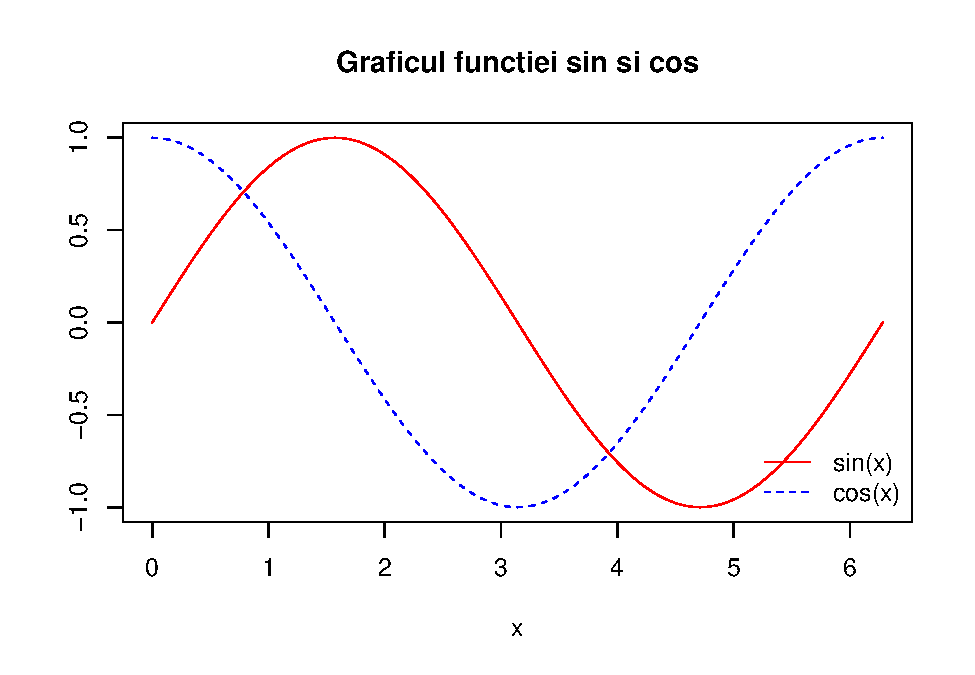
\includegraphics{Lab_2_files/figure-latex/unnamed-chunk-45-1} \end{center}

Un al doilea exemplu ar putea consta în afișarea diagramei de
împrăștiere a mașinilor din setul de date \texttt{mtcars} în funcție de
variabilele \texttt{mpg} și \texttt{wt} în care punctele sunt colorate
în raport cu numărul de cilindrii (4, 6, sau 8), respectiv cu
\emph{roșu}, \emph{orange} și \emph{albastru} și în care afișăm numelor
mașinilor care au transmisie manuală (\texttt{am\ =\ 1}):

\begin{Shaded}
\begin{Highlighting}[]
\KeywordTok{plot}\NormalTok{(mtcars}\OperatorTok{$}\NormalTok{mpg, mtcars}\OperatorTok{$}\NormalTok{wt,}
     \DataTypeTok{col =} \StringTok{"red"}\NormalTok{, }
     \DataTypeTok{pch =} \DecValTok{16}\NormalTok{,}
     \DataTypeTok{cex =} \FloatTok{1.3}\NormalTok{,}
     \DataTypeTok{bty =} \StringTok{"n"}\NormalTok{,}
     \DataTypeTok{xlab =} \StringTok{"Mile pe Galon"}\NormalTok{,}
     \DataTypeTok{ylab =} \StringTok{"Greutatea"}\NormalTok{, }
     \DataTypeTok{main =} \StringTok{"Graficul variabilelor: MPG vs Weight"}\NormalTok{)}

\KeywordTok{points}\NormalTok{(mtcars}\OperatorTok{$}\NormalTok{mpg[mtcars}\OperatorTok{$}\NormalTok{cyl }\OperatorTok{==}\StringTok{ }\DecValTok{6}\NormalTok{], mtcars}\OperatorTok{$}\NormalTok{wt[mtcars}\OperatorTok{$}\NormalTok{cyl }\OperatorTok{==}\StringTok{ }\DecValTok{6}\NormalTok{],}
       \DataTypeTok{col =} \StringTok{"orange"}\NormalTok{,}
       \DataTypeTok{pch =} \DecValTok{16}\NormalTok{,}
       \DataTypeTok{cex =} \FloatTok{1.3}\NormalTok{)}

\KeywordTok{points}\NormalTok{(mtcars}\OperatorTok{$}\NormalTok{mpg[mtcars}\OperatorTok{$}\NormalTok{cyl }\OperatorTok{==}\StringTok{ }\DecValTok{8}\NormalTok{], mtcars}\OperatorTok{$}\NormalTok{wt[mtcars}\OperatorTok{$}\NormalTok{cyl }\OperatorTok{==}\StringTok{ }\DecValTok{8}\NormalTok{],}
       \DataTypeTok{col =} \StringTok{"blue"}\NormalTok{,}
       \DataTypeTok{pch =} \DecValTok{16}\NormalTok{, }
       \DataTypeTok{cex =} \FloatTok{1.3}\NormalTok{)}

\KeywordTok{abline}\NormalTok{(}\DataTypeTok{h =} \KeywordTok{mean}\NormalTok{(mtcars}\OperatorTok{$}\NormalTok{wt),}
       \DataTypeTok{lty =} \DecValTok{2}\NormalTok{)}

\KeywordTok{abline}\NormalTok{(}\DataTypeTok{v =} \KeywordTok{mean}\NormalTok{(mtcars}\OperatorTok{$}\NormalTok{mpg),}
       \DataTypeTok{lty =} \DecValTok{2}\NormalTok{)}

\KeywordTok{text}\NormalTok{(mtcars}\OperatorTok{$}\NormalTok{mpg[mtcars}\OperatorTok{$}\NormalTok{am }\OperatorTok{==}\StringTok{ }\DecValTok{1}\NormalTok{],}
\NormalTok{     mtcars}\OperatorTok{$}\NormalTok{wt[mtcars}\OperatorTok{$}\NormalTok{am }\OperatorTok{==}\StringTok{ }\DecValTok{1}\NormalTok{], }
     \DataTypeTok{labels =} \KeywordTok{rownames}\NormalTok{(mtcars)[mtcars}\OperatorTok{$}\NormalTok{am }\OperatorTok{==}\StringTok{ }\DecValTok{1}\NormalTok{],}
     \DataTypeTok{pos =} \DecValTok{3}\NormalTok{, }
     \DataTypeTok{cex =} \FloatTok{0.8}\NormalTok{)}

\KeywordTok{legend}\NormalTok{(}\StringTok{"topright"}\NormalTok{, }
       \DataTypeTok{legend =} \KeywordTok{c}\NormalTok{(}\StringTok{"cyl = 4"}\NormalTok{, }\StringTok{"cyl = 6"}\NormalTok{, }\StringTok{"cyl = 8"}\NormalTok{),}
       \DataTypeTok{title =} \StringTok{"Nr. Cilindrii"}\NormalTok{,}
       \DataTypeTok{col =} \KeywordTok{c}\NormalTok{(}\StringTok{"red"}\NormalTok{, }\StringTok{"orange"}\NormalTok{, }\StringTok{"blue"}\NormalTok{),}
       \DataTypeTok{pch =} \KeywordTok{c}\NormalTok{(}\DecValTok{16}\NormalTok{,}\DecValTok{16}\NormalTok{,}\DecValTok{16}\NormalTok{),}
       \DataTypeTok{bty =} \StringTok{"n"}\NormalTok{)}
\end{Highlighting}
\end{Shaded}

\begin{center}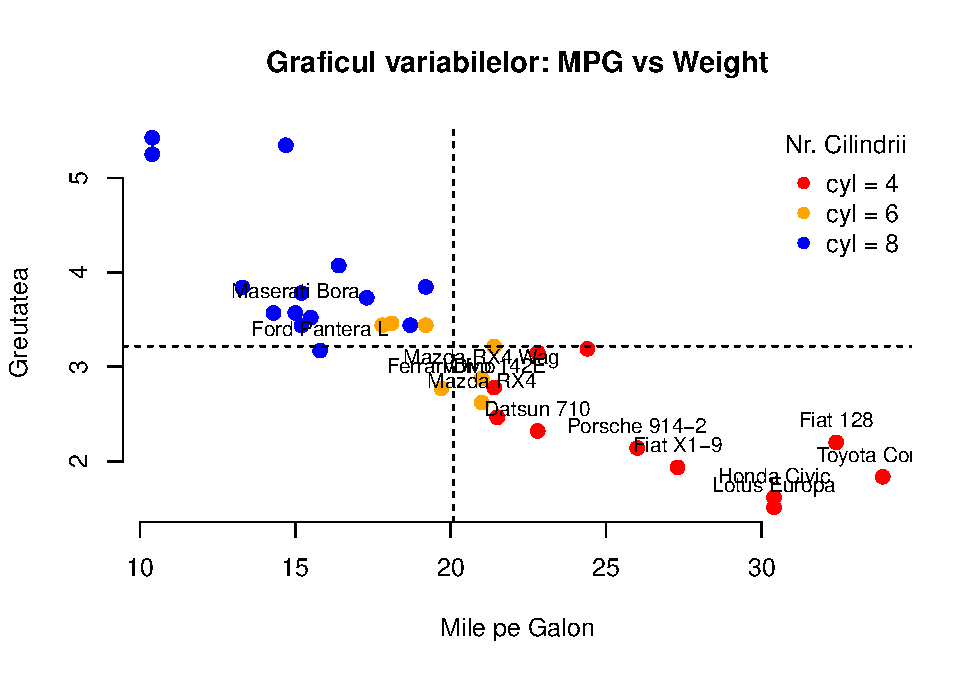
\includegraphics{Lab_2_files/figure-latex/unnamed-chunk-46-1} \end{center}

\subsection{Salvarea figurilor}\label{salvarea-figurilor}

Odată ce am creat un grafic putem să-l salvăm într-un fișier extern.
Pentru aceasta folosim funcțiile \texttt{pdf()}, \texttt{png()} sau
\texttt{jpeg()}. Aceste funcții vor salva figura ca fișier de tip .pdf,
.png sau .jpeg.

\begin{longtable}[]{@{}ll@{}}
\caption{Argumente pentru functiile pdf, jpeg si png}\tabularnewline
\toprule
\begin{minipage}[b]{0.14\columnwidth}\raggedright\strut
Argument\strut
\end{minipage} & \begin{minipage}[b]{0.71\columnwidth}\raggedright\strut
Rezultat\strut
\end{minipage}\tabularnewline
\midrule
\endfirsthead
\toprule
\begin{minipage}[b]{0.14\columnwidth}\raggedright\strut
Argument\strut
\end{minipage} & \begin{minipage}[b]{0.71\columnwidth}\raggedright\strut
Rezultat\strut
\end{minipage}\tabularnewline
\midrule
\endhead
\begin{minipage}[t]{0.14\columnwidth}\raggedright\strut
\texttt{file}\strut
\end{minipage} & \begin{minipage}[t]{0.71\columnwidth}\raggedright\strut
Directorul și numele fișierului sub formă de șir de caractere. De
exemplu, pentru a salva un grafic pe desktop scriem
\texttt{file\ =\ "/Users/.../Desktop/plot.pdf"} pentru un fișier
pdf.\strut
\end{minipage}\tabularnewline
\begin{minipage}[t]{0.14\columnwidth}\raggedright\strut
\texttt{width,\ height}\strut
\end{minipage} & \begin{minipage}[t]{0.71\columnwidth}\raggedright\strut
Dimensiunea graficului final în inchi.\strut
\end{minipage}\tabularnewline
\begin{minipage}[t]{0.14\columnwidth}\raggedright\strut
\texttt{dev.off()}\strut
\end{minipage} & \begin{minipage}[t]{0.71\columnwidth}\raggedright\strut
Acesta nu este un argument al funcțiilor \texttt{pdf()} și
\texttt{jpeg()}. Trebuie executat acest cod după ce trasarea graficului
a fost efectuată pentru a finaliza crearea imaginii.\strut
\end{minipage}\tabularnewline
\bottomrule
\end{longtable}

Pentru a salva o imagine avem de parcurs următorii pași:

\begin{enumerate}
\def\labelenumi{\arabic{enumi}.}
\tightlist
\item
  Execută funcțiile \texttt{pdf()} sau \texttt{jpeg()} cu argumentele
  \texttt{file,\ width,\ height}.
\item
  Execută codul care generează figura (e.g.
  \texttt{plot(x\ =\ 1:10,\ y\ =\ 1:10)})
\item
  Completează scrierea fișierului prin execuția comenzii
  \texttt{dev.off()}. Această comandă spune R-ului că am finalizat
  crearea fișierului.
\end{enumerate}

\begin{Shaded}
\begin{Highlighting}[]
\CommentTok{# Pasul 1}
\KeywordTok{pdf}\NormalTok{(}\DataTypeTok{file =} \StringTok{"/Users/.../Desktop/MyPlot.pdf"}\NormalTok{,   }\CommentTok{# directorul cu fisierul }
    \DataTypeTok{width =} \DecValTok{4}\NormalTok{, }\CommentTok{# latimea in inchi}
    \DataTypeTok{height =} \DecValTok{4}\NormalTok{) }\CommentTok{# inaltimea in inchi}

\CommentTok{# Pasul 2}
\KeywordTok{plot}\NormalTok{(}\DataTypeTok{x =} \DecValTok{1}\OperatorTok{:}\DecValTok{10}\NormalTok{, }
     \DataTypeTok{y =} \DecValTok{1}\OperatorTok{:}\DecValTok{10}\NormalTok{)}
\KeywordTok{abline}\NormalTok{(}\DataTypeTok{v =} \DecValTok{0}\NormalTok{) }
\KeywordTok{text}\NormalTok{(}\DataTypeTok{x =} \DecValTok{0}\NormalTok{, }\DataTypeTok{y =} \DecValTok{1}\NormalTok{, }\DataTypeTok{labels =} \StringTok{"Ceva text aleator"}\NormalTok{)}

\CommentTok{# Pasul 3}
\KeywordTok{dev.off}\NormalTok{()}
\end{Highlighting}
\end{Shaded}


\end{document}
